\hypertarget{Edge Intelligence}{%
	\chapter{Edge Intelligence}\label{ch:edgeintelligence}}
%\thispagestyle{fancy}

\acrfull{ei} brings \gls{ai} closer to the user by the deployment of \gls{ai}-powered applications and services on the edge of the network. Edge \gls{ai} is one of the Top Trends on the Gartner Hype Cycle for Artificial Intelligence in 2019 \cite{goasduff_top_2019}. Section \ref{sec:ei-background} explains the motivation and background of \gls{ei}. Section \ref{sec:ei-architecture} describes edge-centric architectures for \gls{dnn} inference. Section \ref{sec:ei-fast-inference} presents related work, i.e., enabling technologies for fast inference.

\section{Background}\label{sec:ei-background}

The primary objective of \gls{ei} is to enable \gls{ai} for mobile, \gls{iot}, and other applications on the edge of the network. Progress within \gls{ai} and \gls{ml} has been pushed by achievements using \gls{dnn}s, i.e. \gls{dl} for \acrfull{cv} and \gls{nlp} \cite{stoica_berkeley_2017}. State-of-the-art \gls{dnn}s have been too computationally expensive to run anywhere else \cite{zhou_edge_2019} than in the cloud. The improvement of \gls{dnn}s have mostly been impacted by research in training deeper models with the ability to learn features of increasing complexity. The winner of ImageNet Challenge exemplifies the tendency; within only four years have the number of layers grown from 8 to 152 layers \cite{russakovsky_imagenet_2015}. Increasingly deeper models have hindered the deployment of intelligent services onto mobile and \gls{iot} devices, which have made cloud-offloading inevitable. Running algorithms in large-scale data centers come with the side-effect of introducing unpredictable communication delays when accessing the public internet \cite{shi_edge_2016}. The additional communication delay from \gls{ci} has made real-time \gls{ai} infeasible for mobile and \gls{iot} devices. Mobile devices are getting more resourceful, and it is not uncommon to have a smartphone equipped with a \gls{gpu} nowadays. The hardware development has lead to studies of more lightweight \gls{dnn} designs. However, these models cannot achieve state-of-the-art performance. Running \gls{dnn}s on-device is energy consuming and drains the battery of mobile devices.
\gls{ei} is a compromise, which enables deployment of very deep and demanding state-of-the-art \gls{dnn}s on edge servers. Offloading the inference task from the end-device onto edge servers reduces the communication latency compared to cloud-offloading \cite{zhou_edge_2019}. In edge computing, data processing is done in closer proximity to end-users. The shortened communication path leads to a reduction in communication latency \cite{shi_edge_2016}. Edge servers are more powerful than mobile and \gls{iot} devices and can run state-of-the-art models significantly faster. In \cite{karlsen_prototyping_nodate}, edge-based offloading is investigated and shows significant latency improvement compared to both local inference and cloud-offloading. \gls{ei} is a promising compromise to obtain state-of-the-art performance in real-time, necessary for applications such as \gls{ar}/\gls{vr} and Personal Assistant with very stringent latency and reliability requirements \cite{zhou_edge_2019}. Especially for mission-critical applications such as \gls{av}, which require precise, real-time responses \cite{stoica_berkeley_2017}. The real-time \gls{cv} is often defined by classification or object detection at a frame rate between 30-60 frames/s \cite{chen_deep_2019}. \gls{ar} requires between 10-100ms in \emph{motion-to-photons}\cite{chen_deep_2019}. Motion-to-photons is defined as the end-to-end delay from the user moves the field of perception to the display is updated in response to this movement \cite{lavalle_virtual_2019}. Moreover, the \gls{ar}/\gls{vr} headsets will most likely not be able to reserve all available time to run predictive models and would need to offloading such tasks to edge servers \cite{chen_deep_2019}.

The distribution of computing resources envisioned by edge computing stands in sharp contrast to the last decade's centralization of computing resources for cloud computing \cite{shi_edge_2016}. Edge computing is expected to serve the ever-growing number of connected mobile reliably and \gls{iot} devices. A forecast by Cisco estimates 50 billion things to be connected to the internet by 2020 \cite{evans_internet_2011}. With more devices connected to the internet, it will lead to a tremendous explosion in the amount of data generated at the edge, which is expected to reach 850ZB in 2021 \cite{cisco_cisco_2018}. The rapid growth of data generated at the edge is expected to overwhelm the capacity of cloud data centers and will exhaust available bandwidth. Hence processing at the edge is a necessary step in the development and democratizing of \gls{ai} \cite{zhou_edge_2019}.

A concern of \gls{ai} in the cloud is privacy. Data generated by end-devices might be confidential and could contain sensitive information such as speech and faces \cite{chen_deep_2019}. Sensitive information is not allowed to be processed by a data center unless privacy and anonymity can be guaranteed. Edge computing may address this concern as no data leaves the local network since all processing is done at the network edge \cite{chen_deep_2019}. However, edge processing alone does not ensure privacy. Data is still susceptible to interception, as it may be well understood by an adversary. In section \ref{sec:ei-architecture}, it is described how particular edge-centric architectures can promote privacy. 
The survey \citetitle{zhou_edge_2019} by \citet{zhou_edge_2019} review state-of-the-art for \gls{ei}. The survey includes training and inference of \gls{dnn} on the network edge. They review studies for centralized, decentralized, and hybrid training architectures. This project uses a traditional centralized training architecture by training on a single machine. Training architectures will not be elaborated further upon, as the main concern of the thesis is inference latency to provide reliable service for \gls{ai}-driven, time-critical applications. Edge-centric architectures are presented in \ref{sec:ei-architecture}, and related work to obtain faster inference is described in section \ref{sec:ei-fast-inference}. 

\newpage
\section{Edge-centric Architectures} \label{sec:ei-architecture}

Four different edge-centric architectures are illustrated in figure \ref{fig:edge_arch}. \protect\subref{fig:device-based} local on-device inference, \protect\subref{fig:edge-based} edge inference offloading, \protect\subref{fig:edge-device-mode} collaborative edge inference, and \protect\subref{fig:edge-cloud-mode}  collaborative edge-cloud inference. The end-device is illustrated as a smartphone, but could also be an \gls{iot} device.
\begin{figure}
	\begin{minipage}{0.65\linewidth}
		\textbf{\protect\subref{fig:device-based} \textsc{Local on-Device Inference}}
		\color{caption-color} \newline
		The end-device obtains a trained model from the edge server. The end-device acquires input data and process model inference. The performance is only reliant on the computing resources of the end-device since all computation is done on the device. In many cases, the device is not able to run a state-of-the-art model efficiently. Instead, a shallow, less demanding model is run at the cost of accuracy.
	\end{minipage}%
	\hfill
	\begin{minipage}{0.3\linewidth}
		\centering
		\captionsetup[subfigure]{justification=centering}
		\begin{figure}
			\centering
			\subfloat[On-device inference\label{fig:device-based}]{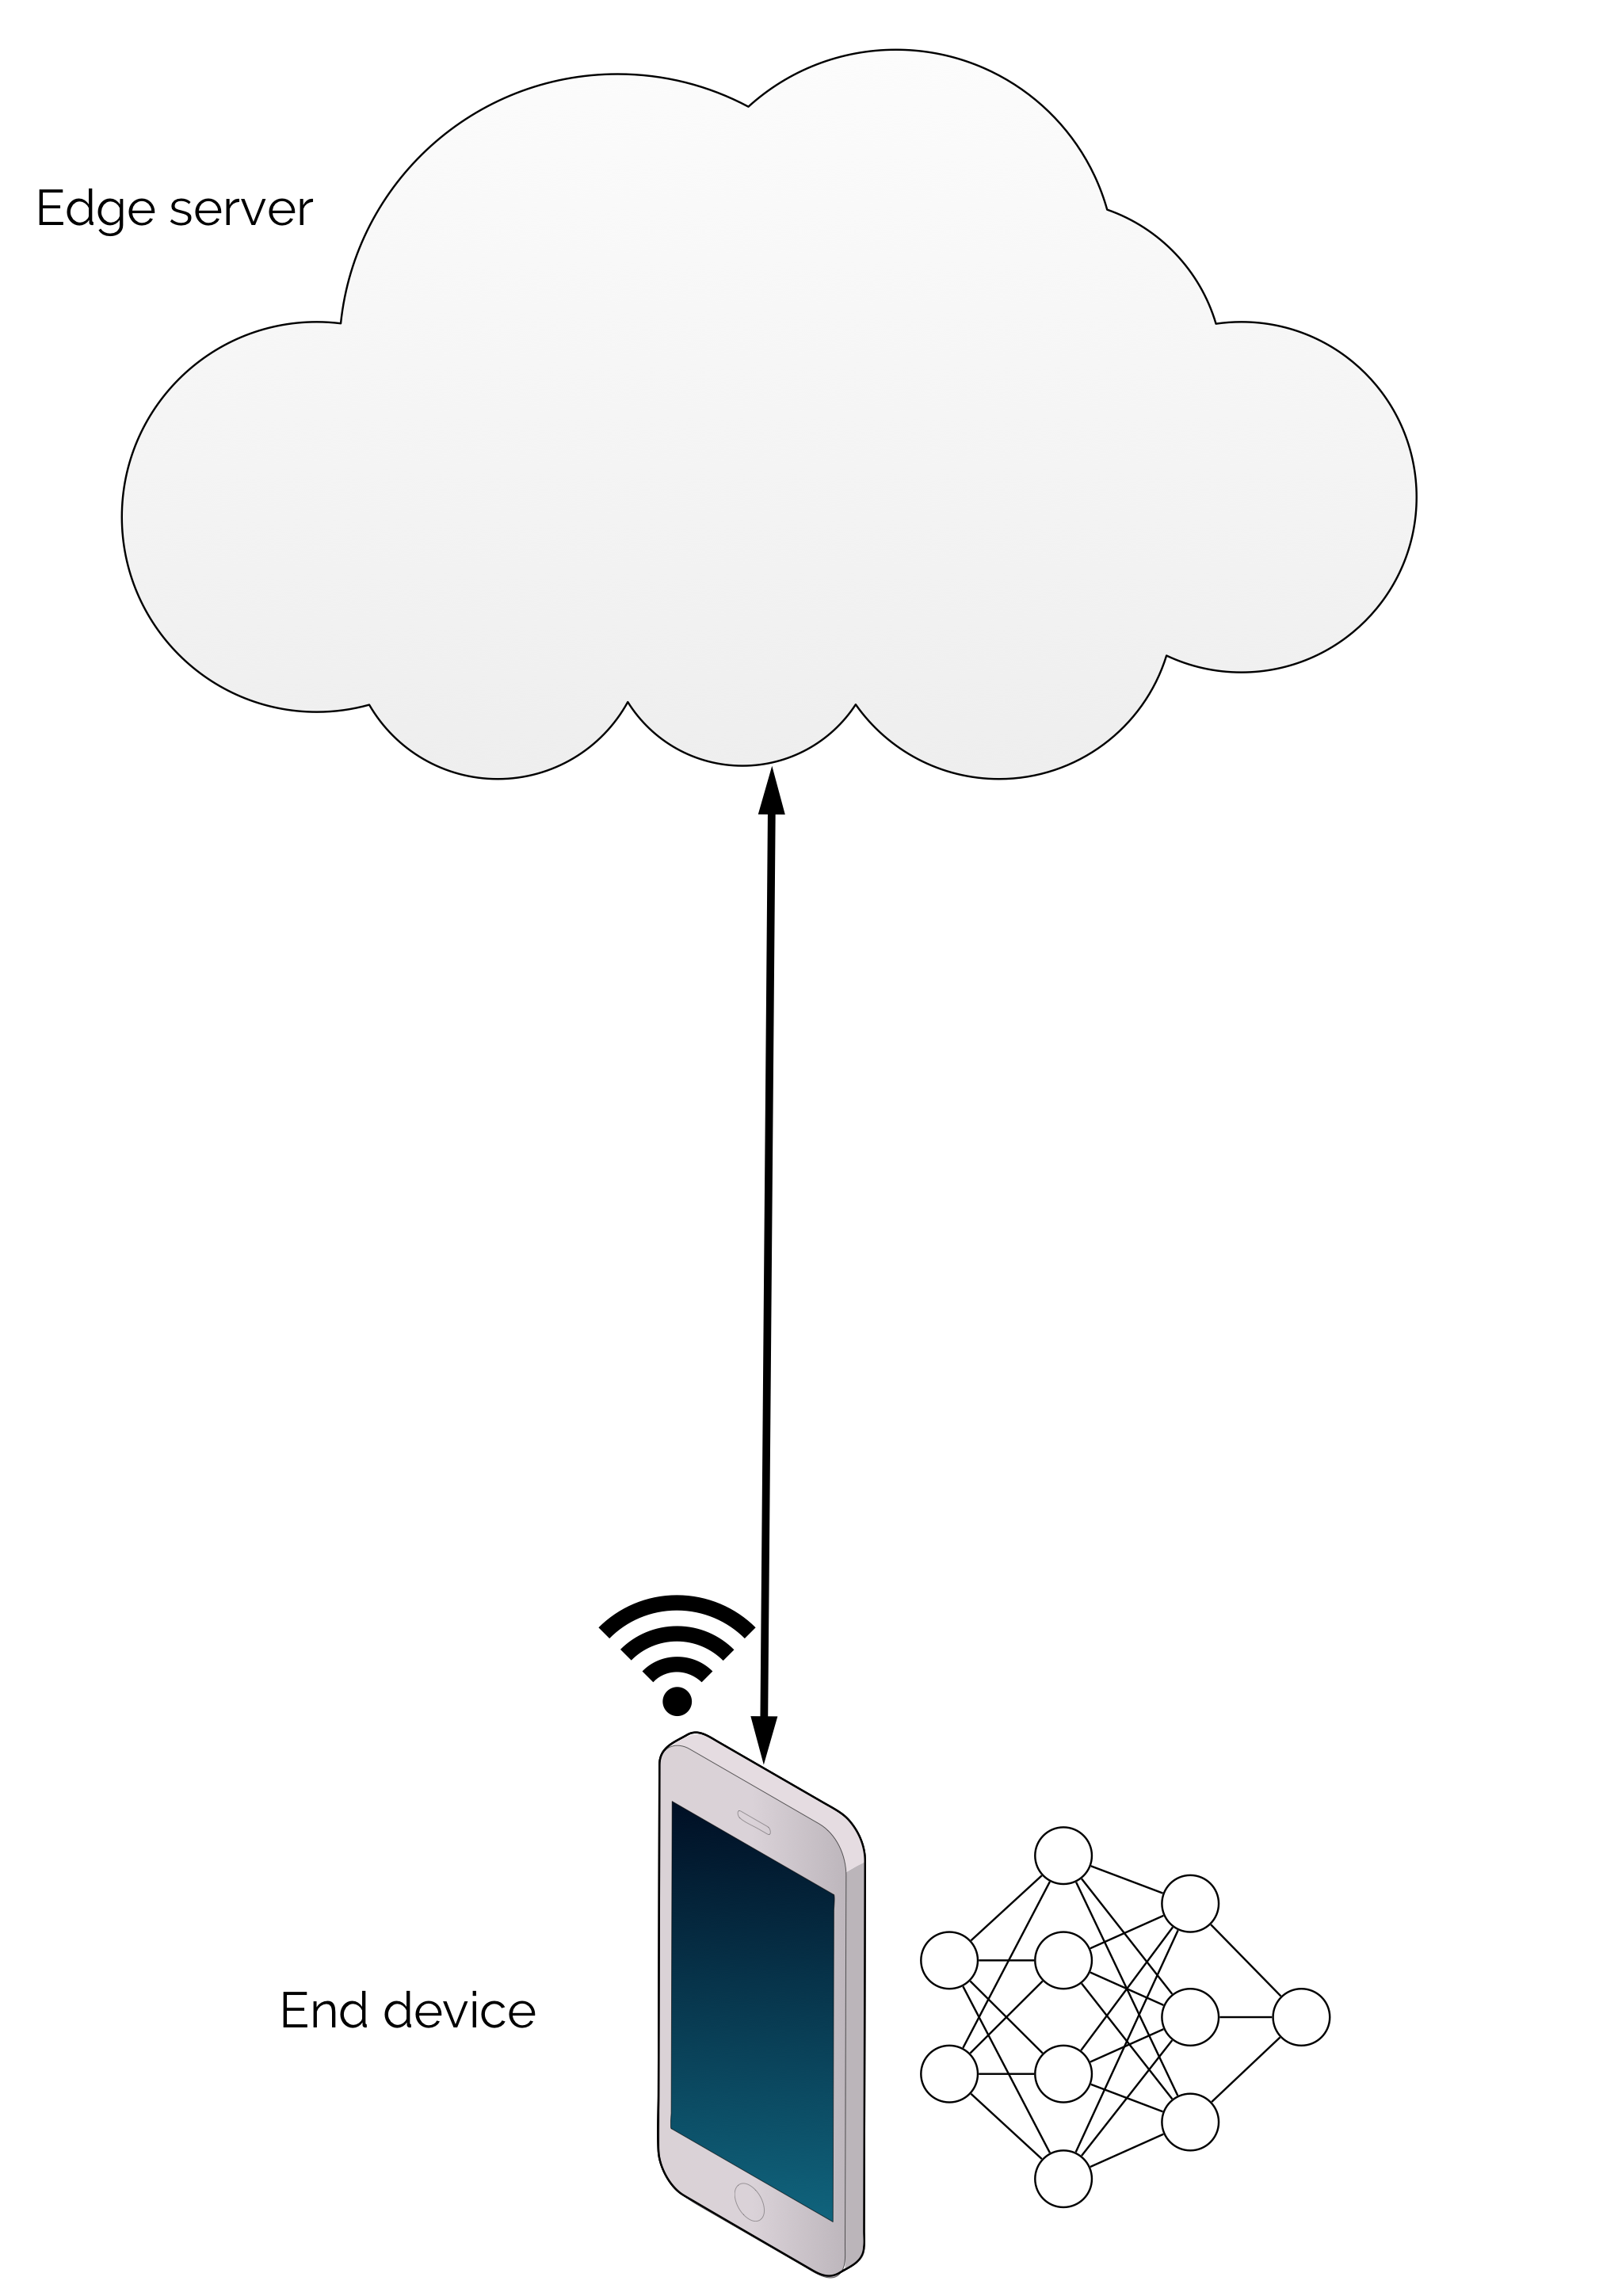
\includegraphics[width=\linewidth]{figures/models/device}}
		\end{figure}
	\end{minipage}
	
	\begin{minipage}{0.3\linewidth}
		\centering
		\begin{figure}
			\centering
			\captionsetup[subfigure]{justification=centering}
			\subfloat[Edge Offloading\label{fig:edge-based}]{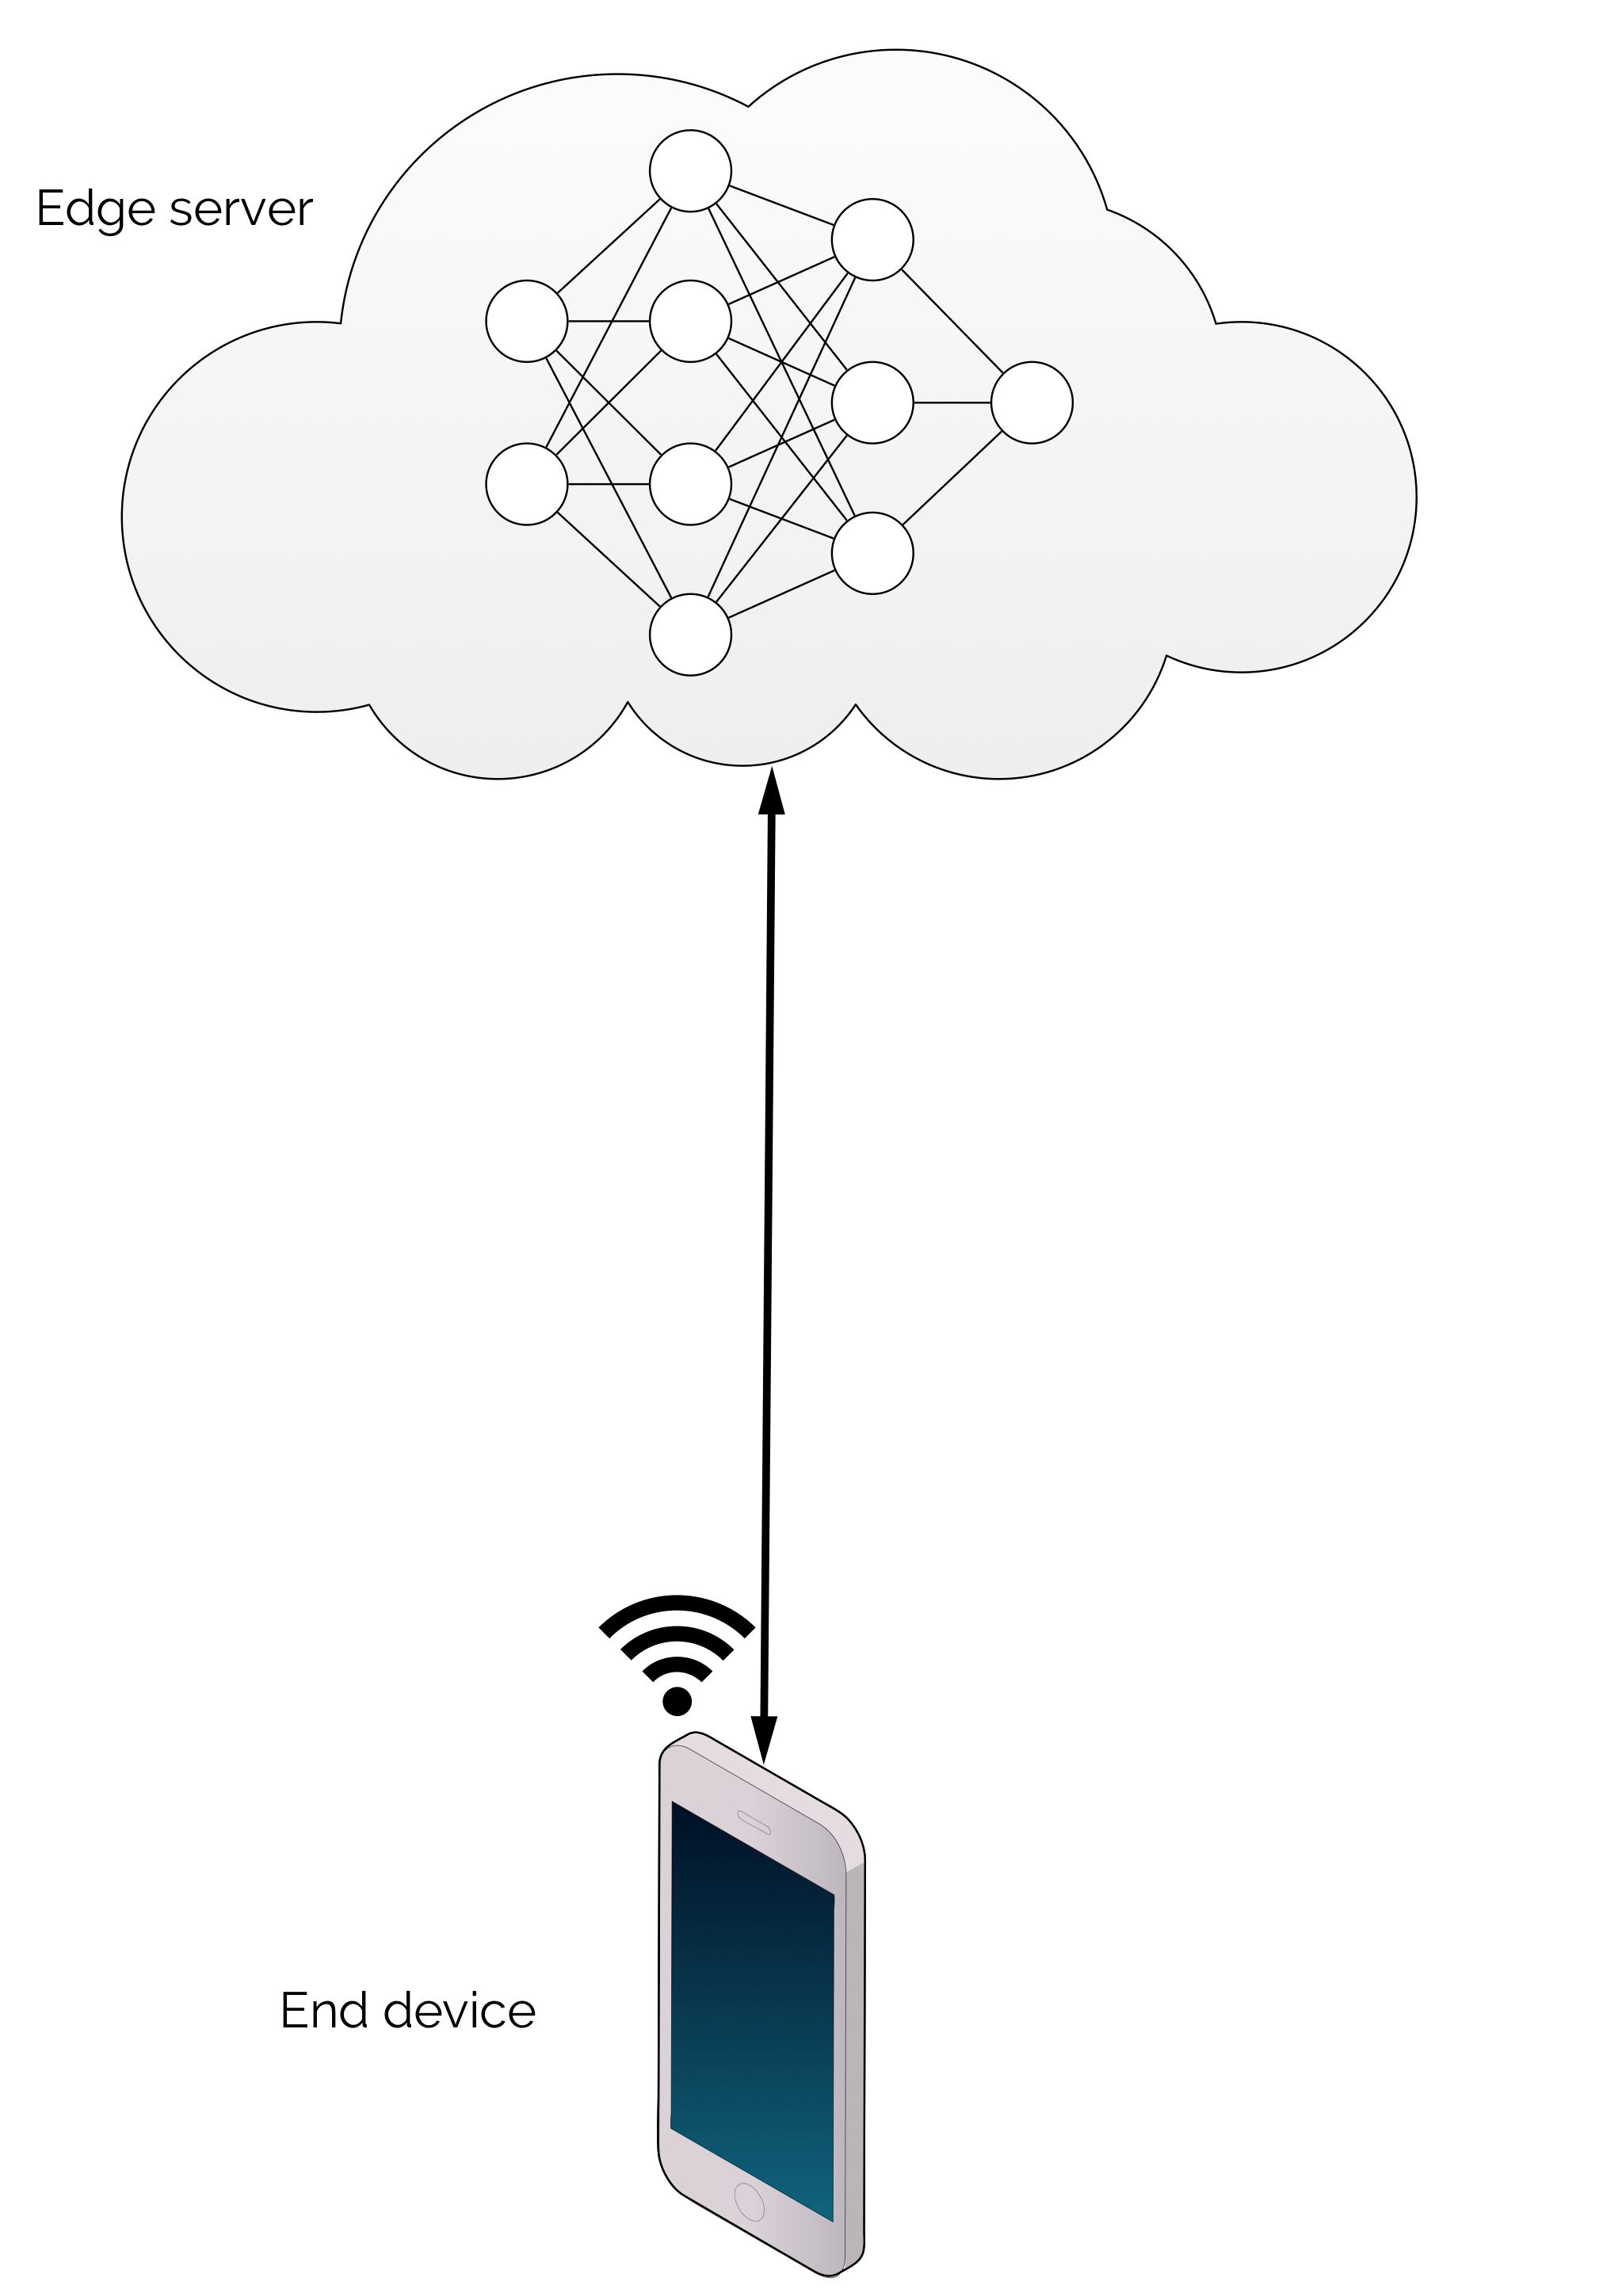
\includegraphics[width=\linewidth]{figures/models/edge}}
		\end{figure}
	\end{minipage}
	\hfill
	\begin{minipage}{0.65\linewidth}
		\textbf{\protect\subref{fig:edge-based} \textsc{Edge Inference Offloading}}
		\color{caption-color} \newline
		Data and model inference is offloaded to the edge. The end device acquires input data and sends it to the edge server. The edge server processes the model inference and sends back the prediction results to the end device. The performance now relies on edge server computing resources and the available network bandwidth between the end-device and the edge server. Note, remote offloading is only sensible, whenever time could be saved, compared to local inference	\end{minipage}
\end{figure}

\begin{figure}
	\begin{minipage}{0.65\linewidth}
		\textbf{\protect\subref{fig:edge-device-mode} \textsc{Collaborative Edge Inference}}
		\color{caption-color} \newline
		The end device acquires input data and performs partial model inference, i.e., only inference some of the layers of the \gls{dnn}. The intermediate data is transferred to the edge server, which infers to the remaining layers of the \gls{dnn}. The performance relies on the computing resource of the end device and the edge server and edge server, and the available network bandwidth between the end-device and the edge server. Collaborative edge promotes privacy, as intermediate features have no apparent meaning for humans, which will improve the confidentiality of the transferred data.   
	\end{minipage}%
	\hfill
	\begin{minipage}{0.3\linewidth}
		\centering
		\captionsetup[subfigure]{justification=centering}
		\begin{figure}
			\centering
			\subfloat[Collaborative Edge Inference\label{fig:edge-device-mode}]{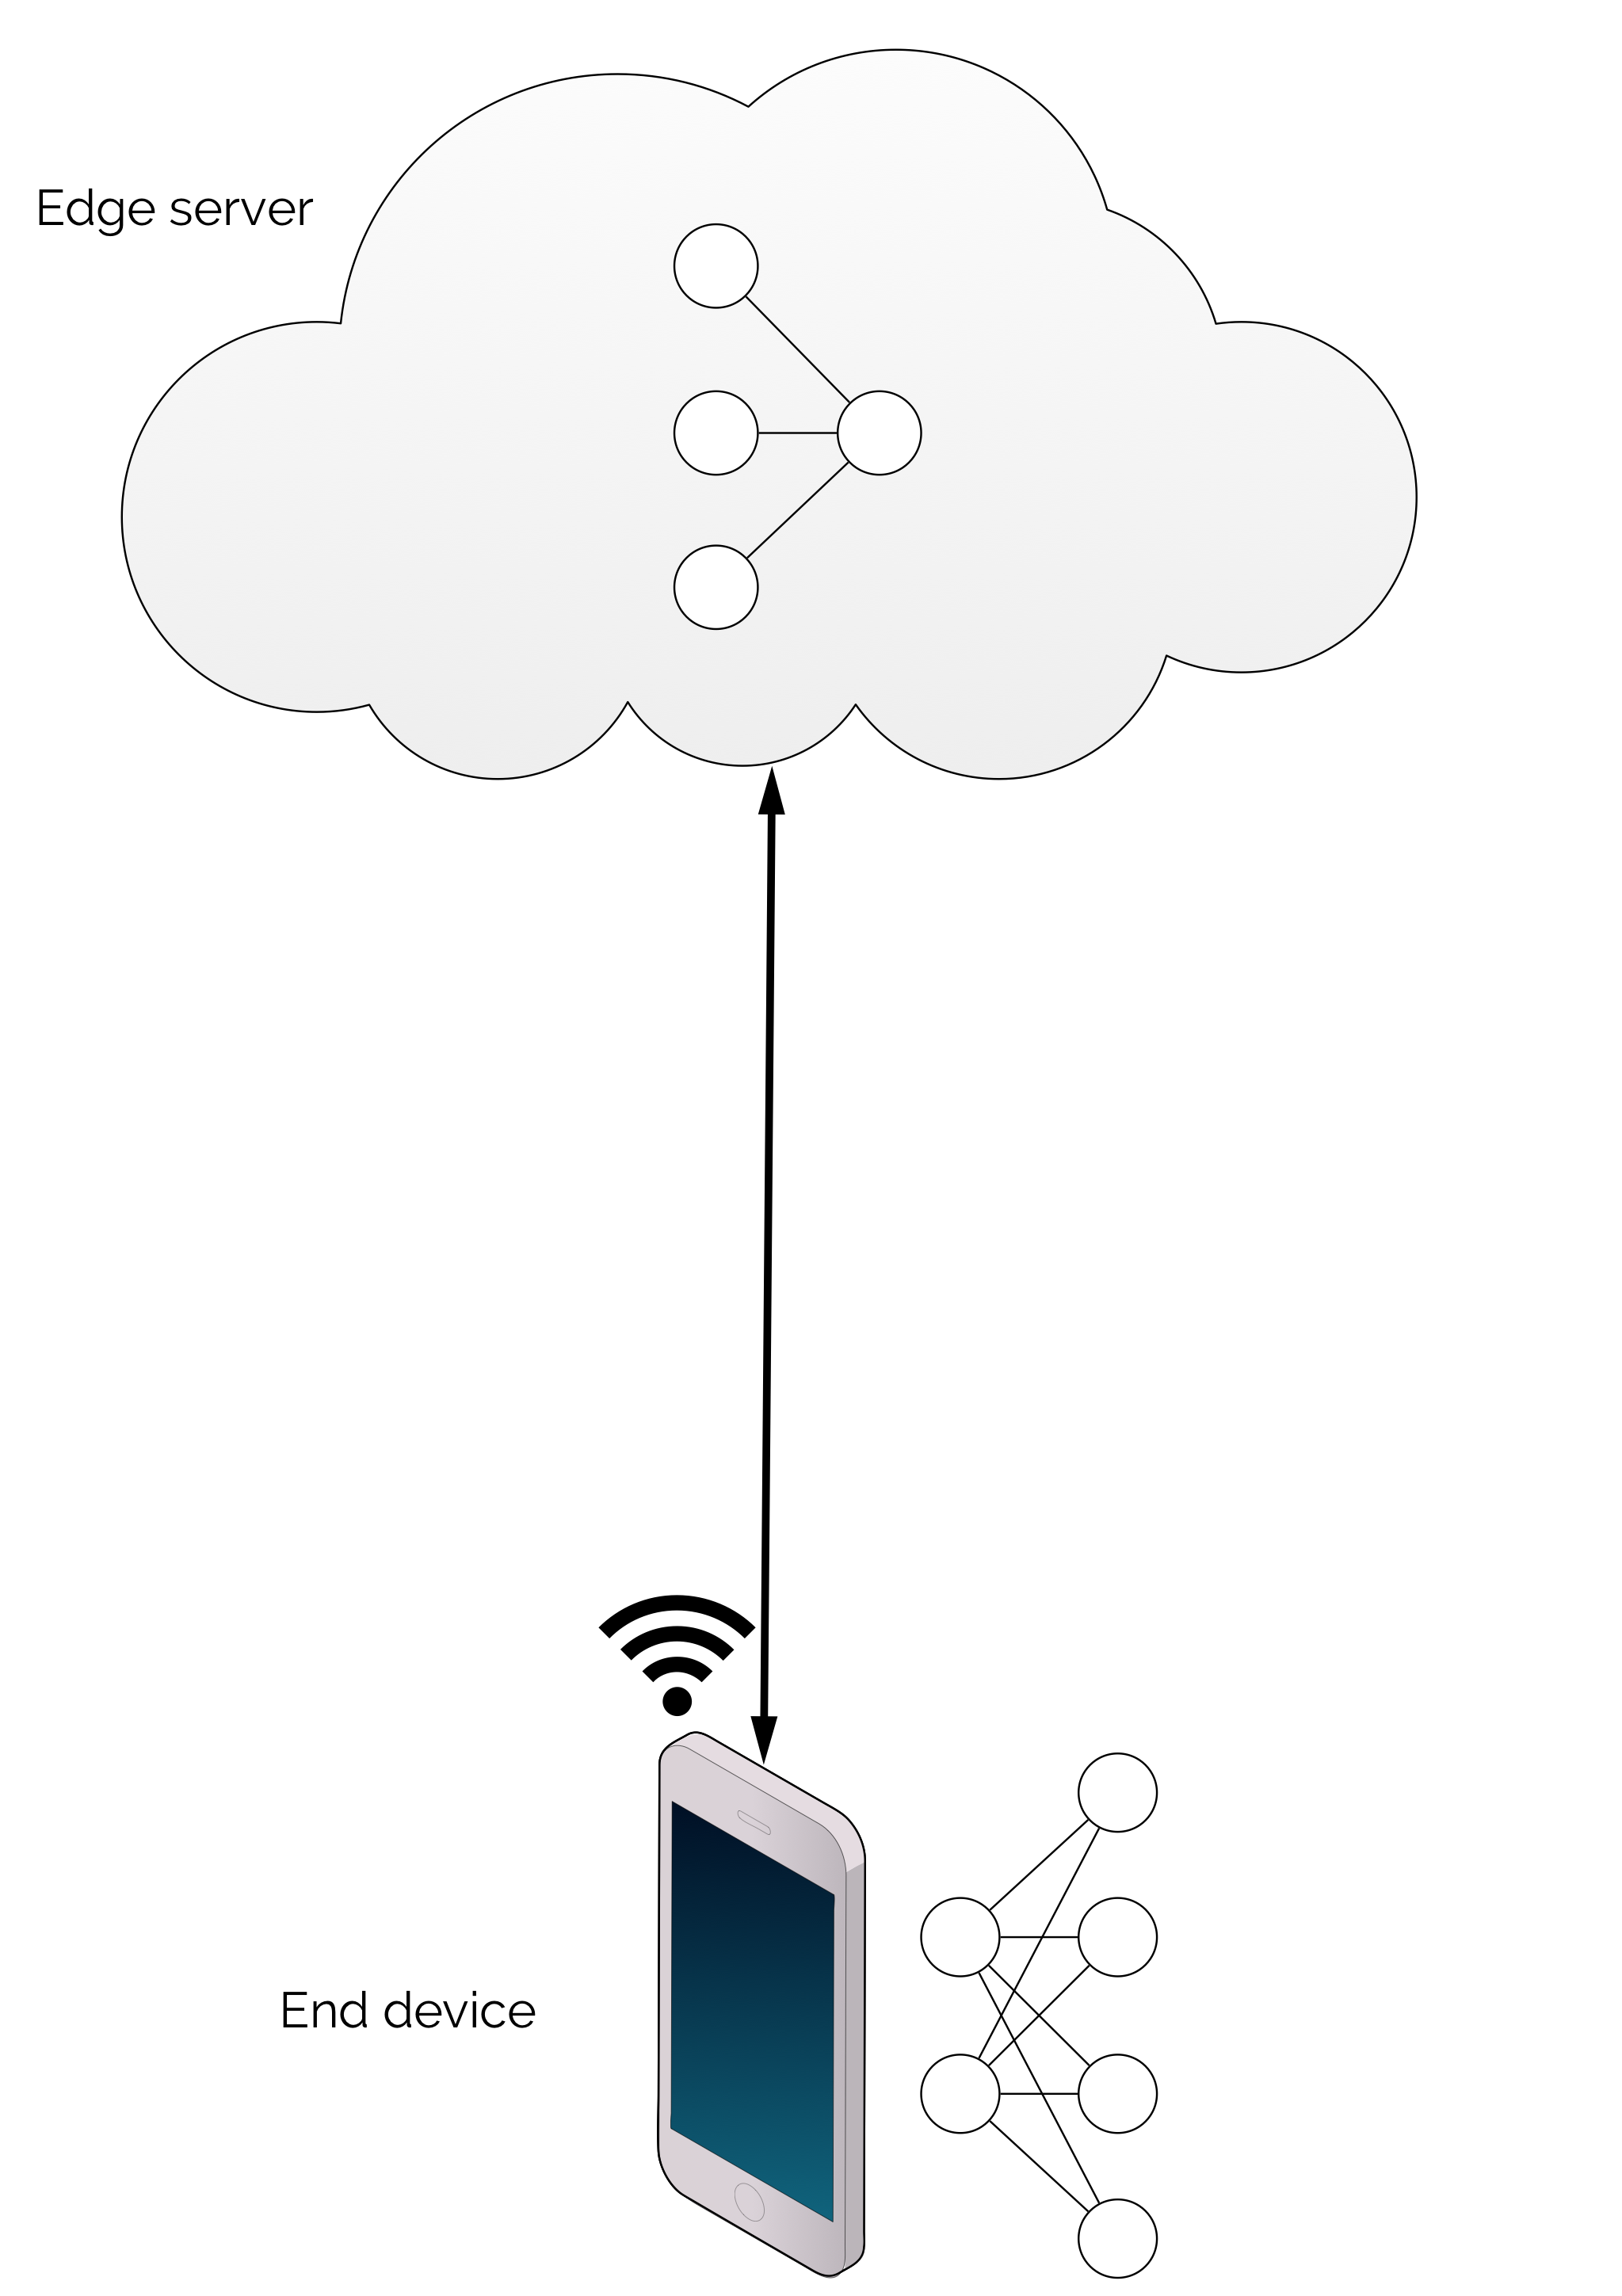
\includegraphics[width=\linewidth]{figures/models/edge_device}}
		\end{figure}
	\end{minipage}
	\vskip 2em
	\begin{minipage}{0.5\linewidth}
		\centering
		\captionsetup[subfigure]{justification=centering}
		\begin{figure}
			\centering
			\subfloat[Collaborative Edge-Cloud Inference\label{fig:edge-cloud-mode}]{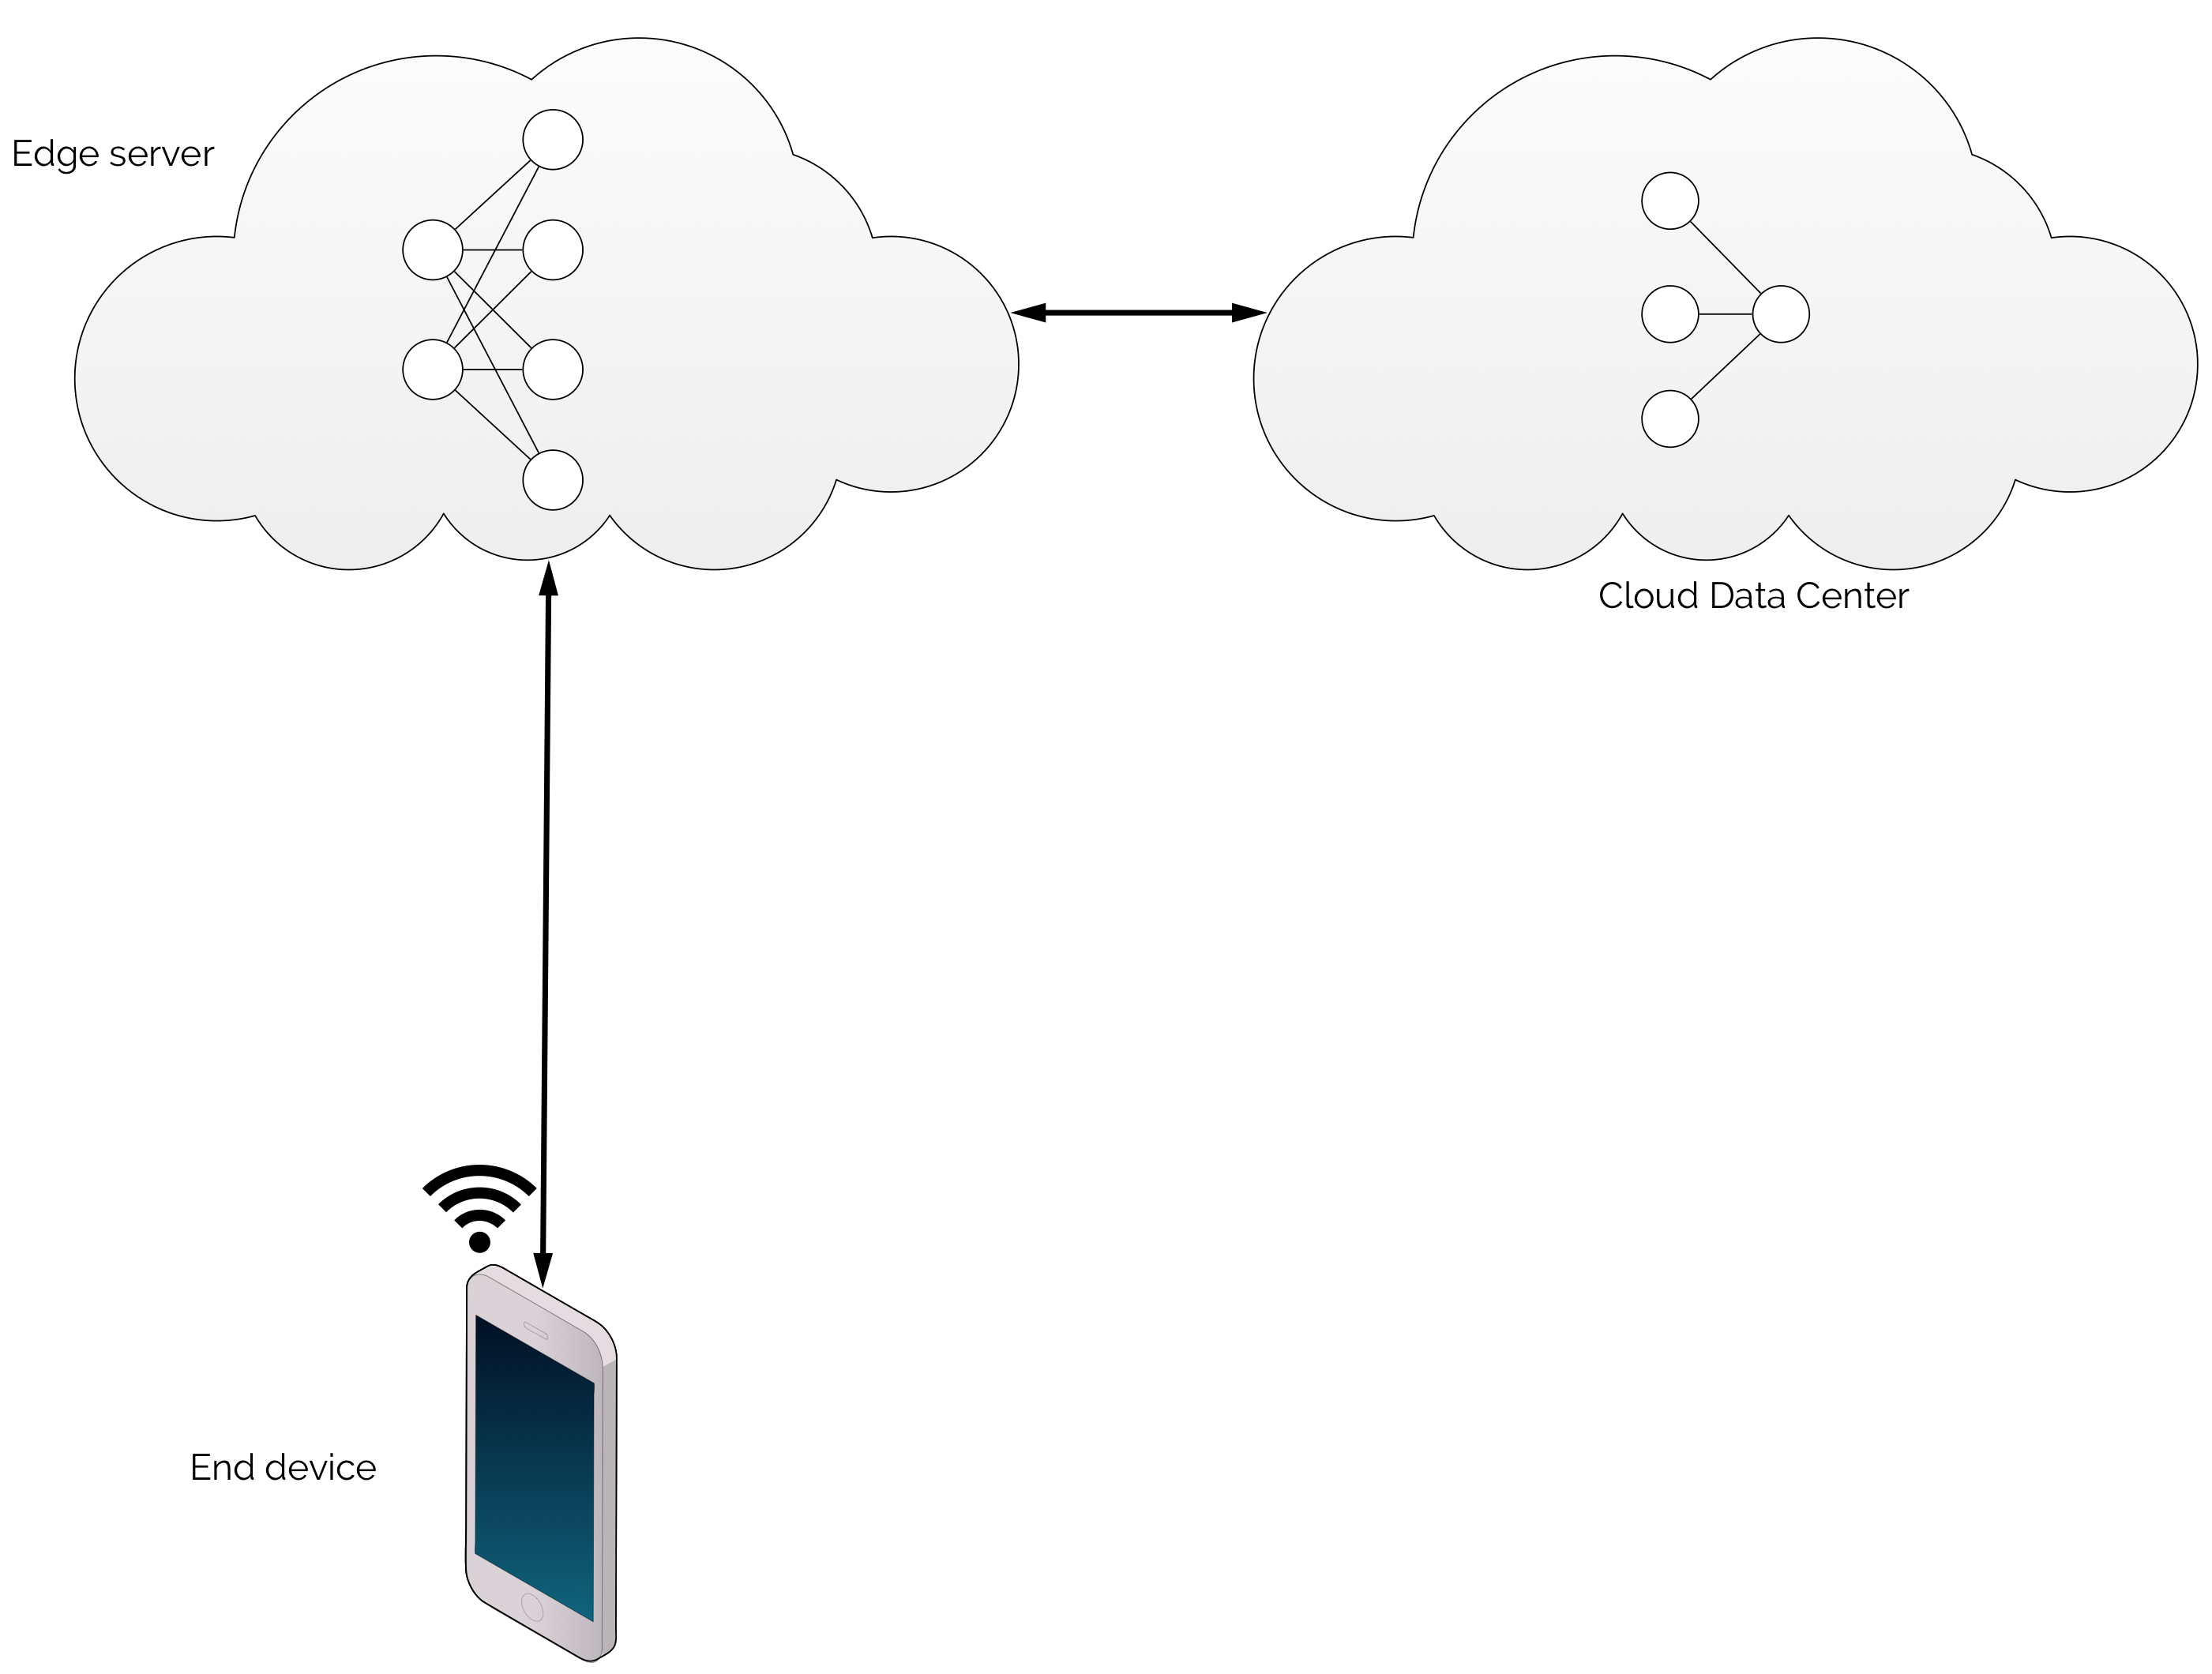
\includegraphics[width=\linewidth]{figures/models/edge_cloud}}
		\end{figure}
	\end{minipage}
	\hfill
	\begin{minipage}{0.45\linewidth}
		\textbf{\protect\subref{fig:edge-cloud-mode} \textsc{Collaborative Edge-Cloud Inference}}
		\color{caption-color} \newline
		This architecture resembles the collaborative edge inference. However, the layer of the model is partitioned between the edge server and the cloud. The inference relies on computing resources of the edge server and cloud, but not least on the available network bandwidth between edge and cloud. The scheme promotes privacy, however, between edge and cloud and not in the local network on the edge. The two architectures are seen combined in \cite{leroux_cascading_2017, teerapittayanon_distributed_2017} to partition the inference between device, edge, and cloud. 
	\end{minipage}
	\caption[Edge-centric Architectures]{Edge-centric Architectures: \protect\subref{fig:device-based} local on-device inference, \protect\subref{fig:edge-based} edge inference offloading, \protect\subref{fig:edge-device-mode} collaborative edge inference, and \protect\subref{fig:edge-cloud-mode}  collaborative edge-cloud inference. }
	\label{fig:edge_arch}
\end{figure}

In the next section, first is related work for local on-device inference and edge inference offloading presented, where all processing is done solely by one peer. Secondly, is related work for collaborative inference presented, where the processing is partitioned on the depth-axis between multiple peers. Lastly, is distributed inference presented, where processing is partitioned on the input-axis between multiple peers. 
\section{Fast Inference} \label{sec:ei-fast-inference}
In this section, are enabling technologies for fast inference described. Our main concern is obtaining faster inference on a model-level. Other research directions are, for instance, hardware acceleration for \gls{cpu}s and \gls{gpu}s, and development of \gls{asic} and \gls{fpga}, i.e., specialized hardware such as Google's \gls{tpu} to accelerate training and inferencing \gls{dnn}s. 

We present studies in current literature that operates on a model level, e.g., model design, -compression, -selection, -early exit, and -layer skipping. Additionally, for collaborative inference we present methods to reduce communication delays such as feature compression and other partition architectures. Table \ref{tbl:fast-inference} summarizes the technologies. We omit technologies that operates on an infrastructural level, e.g., edge caching, input filtering, and support for multi-tenancy \cite{zhou_edge_2019}.
\begin{minipage}[t]{\linewidth}
	\begin{footnotesize}
		\begin{longtabu}{>{\bfseries}X[c]|X[l]|X[3l]|X[c]}
			\caption[Fast Inference Related Work]{Enabling technologies categorized by inference architecture. On-device and edge offloading have been collapsed, as both are central processing. Collaborative edge and edge cloud are collapsed, as both are decentral processing. The Distributed inference is decentral, but the partitioning is done in the input-axis.} \label{tbl:fast-inference} \\
			\toprule
			\rowfont{\bfseries}
			Architecture & Technology & Speed-Up method & Works \tabularnewline
			\hline
			\endfirsthead
			\multicolumn{3}{@{}l}{\textbf{\textcolor{black}{Table \ref{tbl:fast-inference}:}} continued}\\
			\toprule
			\rowfont{\bfseries}
			Architecture & Technology & Speed-Up method & Works \tabularnewline
			\hline
			\endhead % all the lines above this will be repeated on every page
			\hline
			\multicolumn{3}{@{}l}{continued \ldots}\\
			\endfoot
			\hline
			\endlastfoot
			On-Device or & Model Design & Innovative layer and operation design & \cite{iandola_squeezenet:_2016,howard_mobilenets:_2017,sandler_mobilenetv2:_2018, zhang_shufflenet:_2017, ma_shufflenet_2018} \tabularnewline
			\tabucline{2-6}
			
			Edge Offloading & Model Compression & Reduce model size by removal of non-contributing neuron weights and connections &  \cite{hinton_distilling_2015,courbariaux_binaryconnect:_2015,courbariaux_binarized_2016,romero_fitnets:_2014} \tabularnewline	
			\tabucline{2-6}
			
			& Model Selection & Reduce depth overhead by selecting smaller model%, May require multiple \gls{dnn} inferences 
			& \cite{bolukbasi_adaptive_2017, tann_flexible_2018, park_big/little_2015} \tabularnewline
			\tabucline{2-6}
			
			& Model Early Exit & Reduce depth overhead using by early exit to use less layers%, No additional inference, Multiple predictions, Possible lack of coarse level features 
			& \cite{leroux_resource-constrained_2015,teerapittayanon_branchynet:_2016, berestizshevsky_sacrificing_2019, kaya_shallow-deep_nodate, huang_multi-scale_2017} \tabularnewline
			\tabucline{2-6}
			& Model Layer Skipping & Reduce depth overhead by skipping layers %Poses Coarse level features, Require additional reinforcement learning of skipping policies 
			& \cite{wang_skipnet:_2017,wu_blockdrop:_2017} \tabularnewline\hline
			
			Collaborative Edge  & Feature Compression & Reduce size of intermediate feature size to reduce communication latency%, Resquires Compression aware training, Additional time to compress 
			& \cite{kang_neurosurgeon:_2017,choi_near-lossless_2018, choi_deep_2018, eshratifar_bottlenet:_2019} \tabularnewline
			\tabucline{2-6}
			
			or Edge-Cloud & Distributed Exits & Reduced depth and communication overhead of offloading using local early exits%, Reduce unnecessary communication efforts, no additional inference task, computation latency overhead from local processing, communication latency if not exiting locally 
			& \cite{leroux_cascading_2017,teerapittayanon_distributed_2017, li_edge_2018} \tabularnewline\hline
			
			Distributed & Input-wise partitioning & Distributing workload to multiple peers, beneficial for constraint devices not able to run inference%, can collaborate to solve the task, Requires Orchestration and Synchronization, Data dependence between peers 
			& \cite{mao_modnn:_2017, zhao_deepthings:_2018}
			\tabularnewline
			
			\bottomrule
		\end{longtabu}
	\end{footnotesize}
\end{minipage}

\subsection{Local On-device Inference and Edge Inference Offloading}

In this section, we present studies aimed at centralized inference.

\begin{enumdescript}
	\item[Model Design] To improve inference latency, studies have been made in designing \gls{dnn}s, which reduces the size of the model. Smaller models reduce the memory footprint and run more efficiently on mobile and \gls{iot} devices. Most research addresses ways to reduce the number of parameters, such as SqueezeNet \cite{iandola_squeezenet:_2016}, that downsamples the data size for a thinner network. Others propose creating more efficient models that reduce the number of \acrshort{flop}s. MobileNets \cite{howard_mobilenets:_2017,sandler_mobilenetv2:_2018} decomposes the convolution filters into simpler operations, thus reduces the number of computations for the model. ShuffleNets \cite{zhang_shufflenet:_2017, ma_shufflenet_2018} uses a point-wise convolution operation and channel shuffling to reduce the number of computations. Commonly, all these models are less accurate compared to the state-of-the-art model, but far more efficient \cite{bianco_benchmark_2018}. 
		
	\item[Model compression] Pruning is a widespread compression technique. It is used to create sparse networks by removing the least contributing neurons and connections. Pruning has shown significant speed-ups with only a small loss in accuracy \cite{zhou_edge_2019}. The impact of compression is application dependent and can be applied to any pre-trained \gls{dnn}. Additionally, it can be used in combination with other techniques \cite{cheng_survey_2017}.
	
	\begin{minipage}[t]{\linewidth}
		\centering
		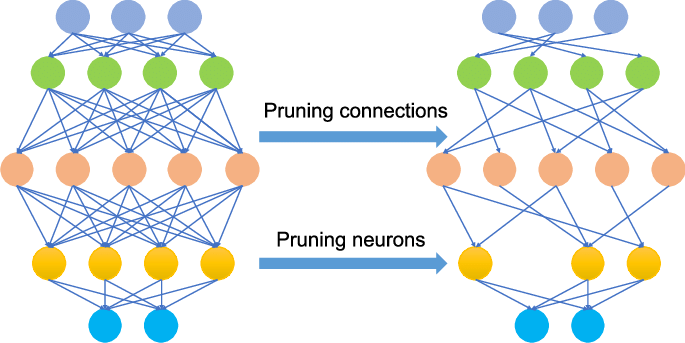
\includegraphics[width=.4\linewidth]{figures/articles/Pruning-a-neural-network}
		\captionof{figure}[\gls{dnn} Pruning]{Pruning connection and neurons source: \citetitle{chen_deep_2019} \cite{chen_deep_2019}}
	\end{minipage}
	
	Quantization is a compression technique by using a more compact representation of network weights and activations, i.e., 16-bit floating-point instead of 32-bit floating-point \cite{cheng_survey_2017}. The extreme case is binarization, where weights and activations are learned as a binary representation. In BinaryConnect \cite{courbariaux_binaryconnect:_2015} and \gls{bnn} \cite{courbariaux_binarized_2016}, arithmetic operations are replaced with bit-wise operations, thus significantly improving the power-efficiency and inference latency. However, using binary weights for the extremely deep networks have shown significant degradation of model accuracy \cite{cheng_survey_2017}.
	
	In \cite{hinton_distilling_2015}, \gls{kd} is proposed. \gls{kd} is a framework to train \gls{dnn} in a student-teacher paradigm. The student network is penalized using the output of an ensemble of teacher networks. \gls{kd} can be viewed as compression of the ensemble of teacher networks into the student network \cite{cheng_survey_2017}. 
	In \cite{romero_fitnets:_2014}, FitNet is proposed. FitNet is a method to train thinner and shallower student networks using a deeper teacher network. In FitNet, the student network learns to mimic the teacher network. However, this approach requires the softmax loss function, which limits its usage \cite{cheng_survey_2017}.  
	
	\item[Model Selection] Model selection aims to reduce inference by selecting an appropriately deep model. If a shallow model can produce satisfying predictions, time is saved by not running an unnecessarily deep model. In \cite{bolukbasi_adaptive_2017}, an adaptive model selection framework is proposed. The framework stacks three \gls{dnn}s with increasing depth and accuracy; \gls{alexnet}, \gls{googlenet}, and \gls{resnet}50. 
	
	\begin{minipage}[t]{\linewidth}
		\centering                           
		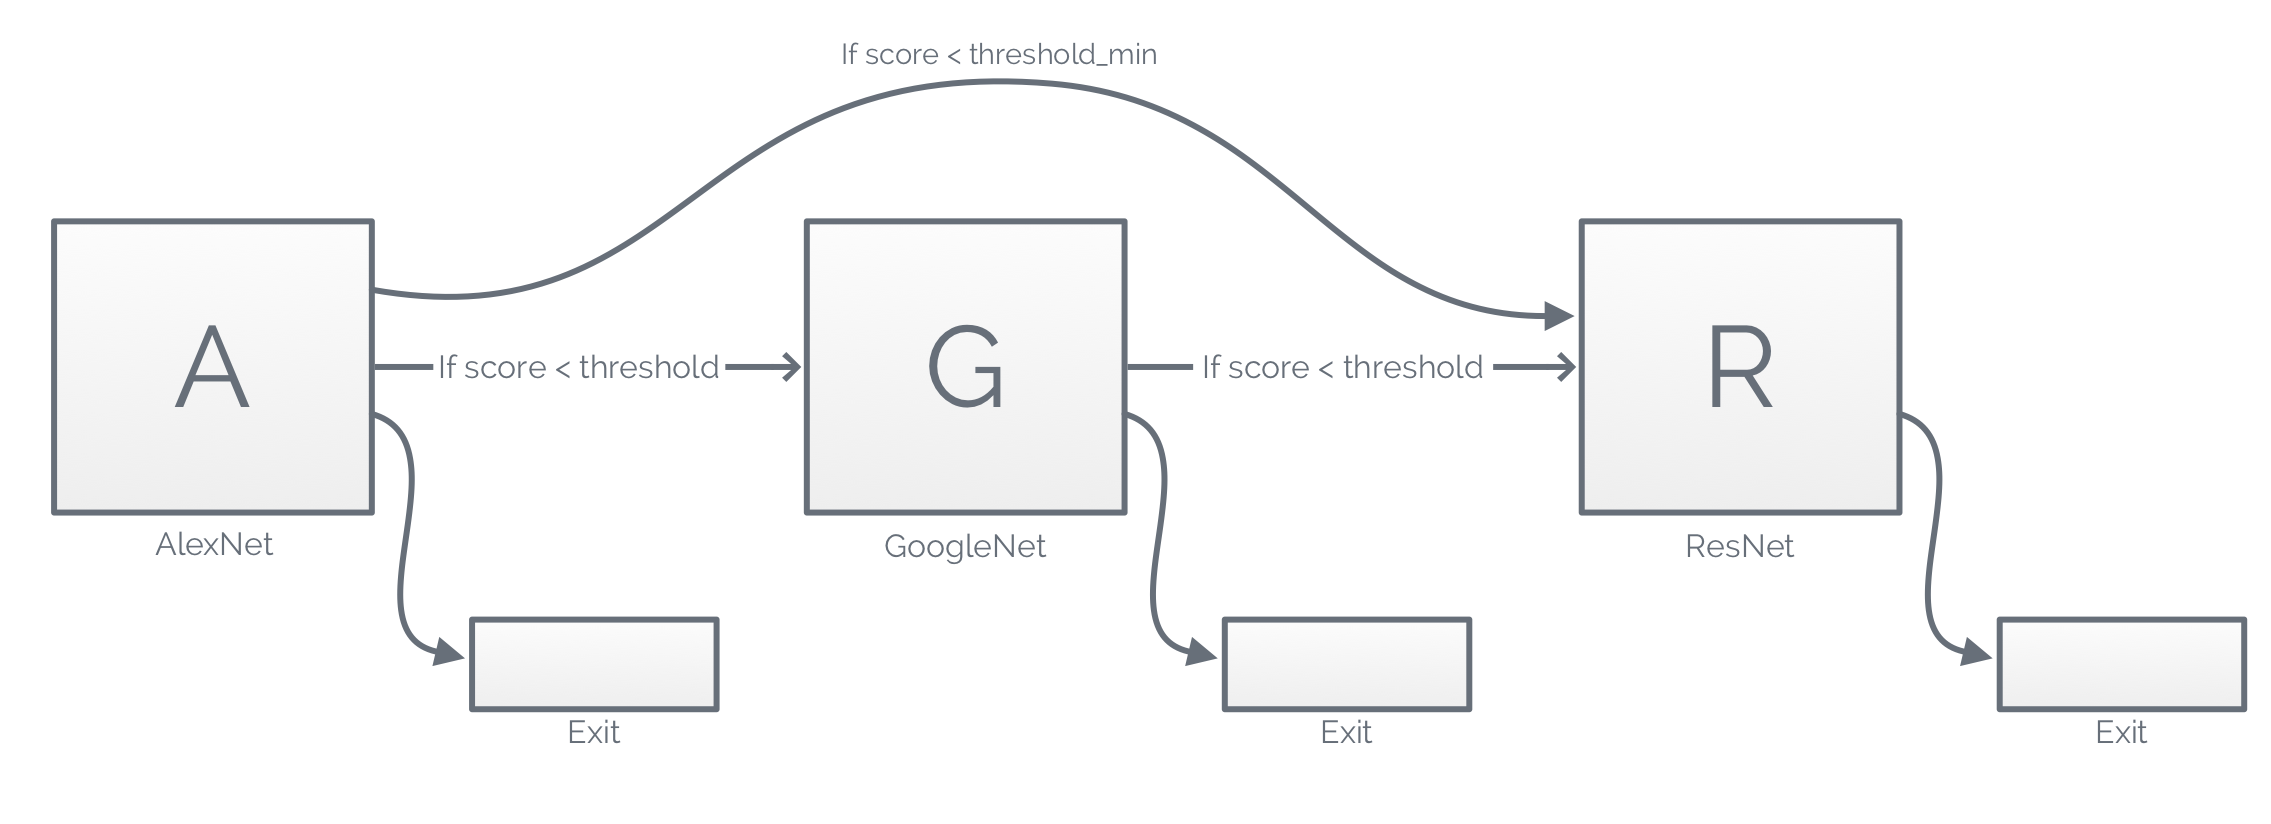
\includegraphics[width=.8\linewidth]{figures/models/adaptive}
		\captionof{figure}[Adaptive Neural Network]{Adaptive Neural Network using model selection}
	\end{minipage}
	
	The input is inferred in \gls{alexnet}; the prediction is accepted if the confidence score is satisfying. If not, a decision is made to infer in either \gls{googlenet} or \gls{resnet}50, depending on a confidence threshold. However, if the sample is inferred to \gls{googlenet} and the confidence is still unsatisfying, the sample is inferred in \gls{resnet}50 for final prediction. In \cite{tann_flexible_2018}, they propose stacking an ensemble of networks in the same manner. Both works show improvement in the average inference time with only a small reduction in accuracy, depending on the confidence threshold. For hard samples, the inference time increases, since multiple models are introduced. Multiple models increase computational cost and memory consumption. Thus, such a model selection approach seems overwhelming to introduce on a constraint end device. 	
	To obtain faster inference, Big/Little \gls{dnn} \cite{park_big/little_2015} implements a hybrid architecture of device and selective offloading for edge processing. It runs a shallower, albeit less accurate model on-device, and a deep and more accurate model on the edge server, as illustrated by figure \ref{fig:big/little-dnn}. 
	
	\begin{minipage}[t]{\linewidth}    
		\centering                          
		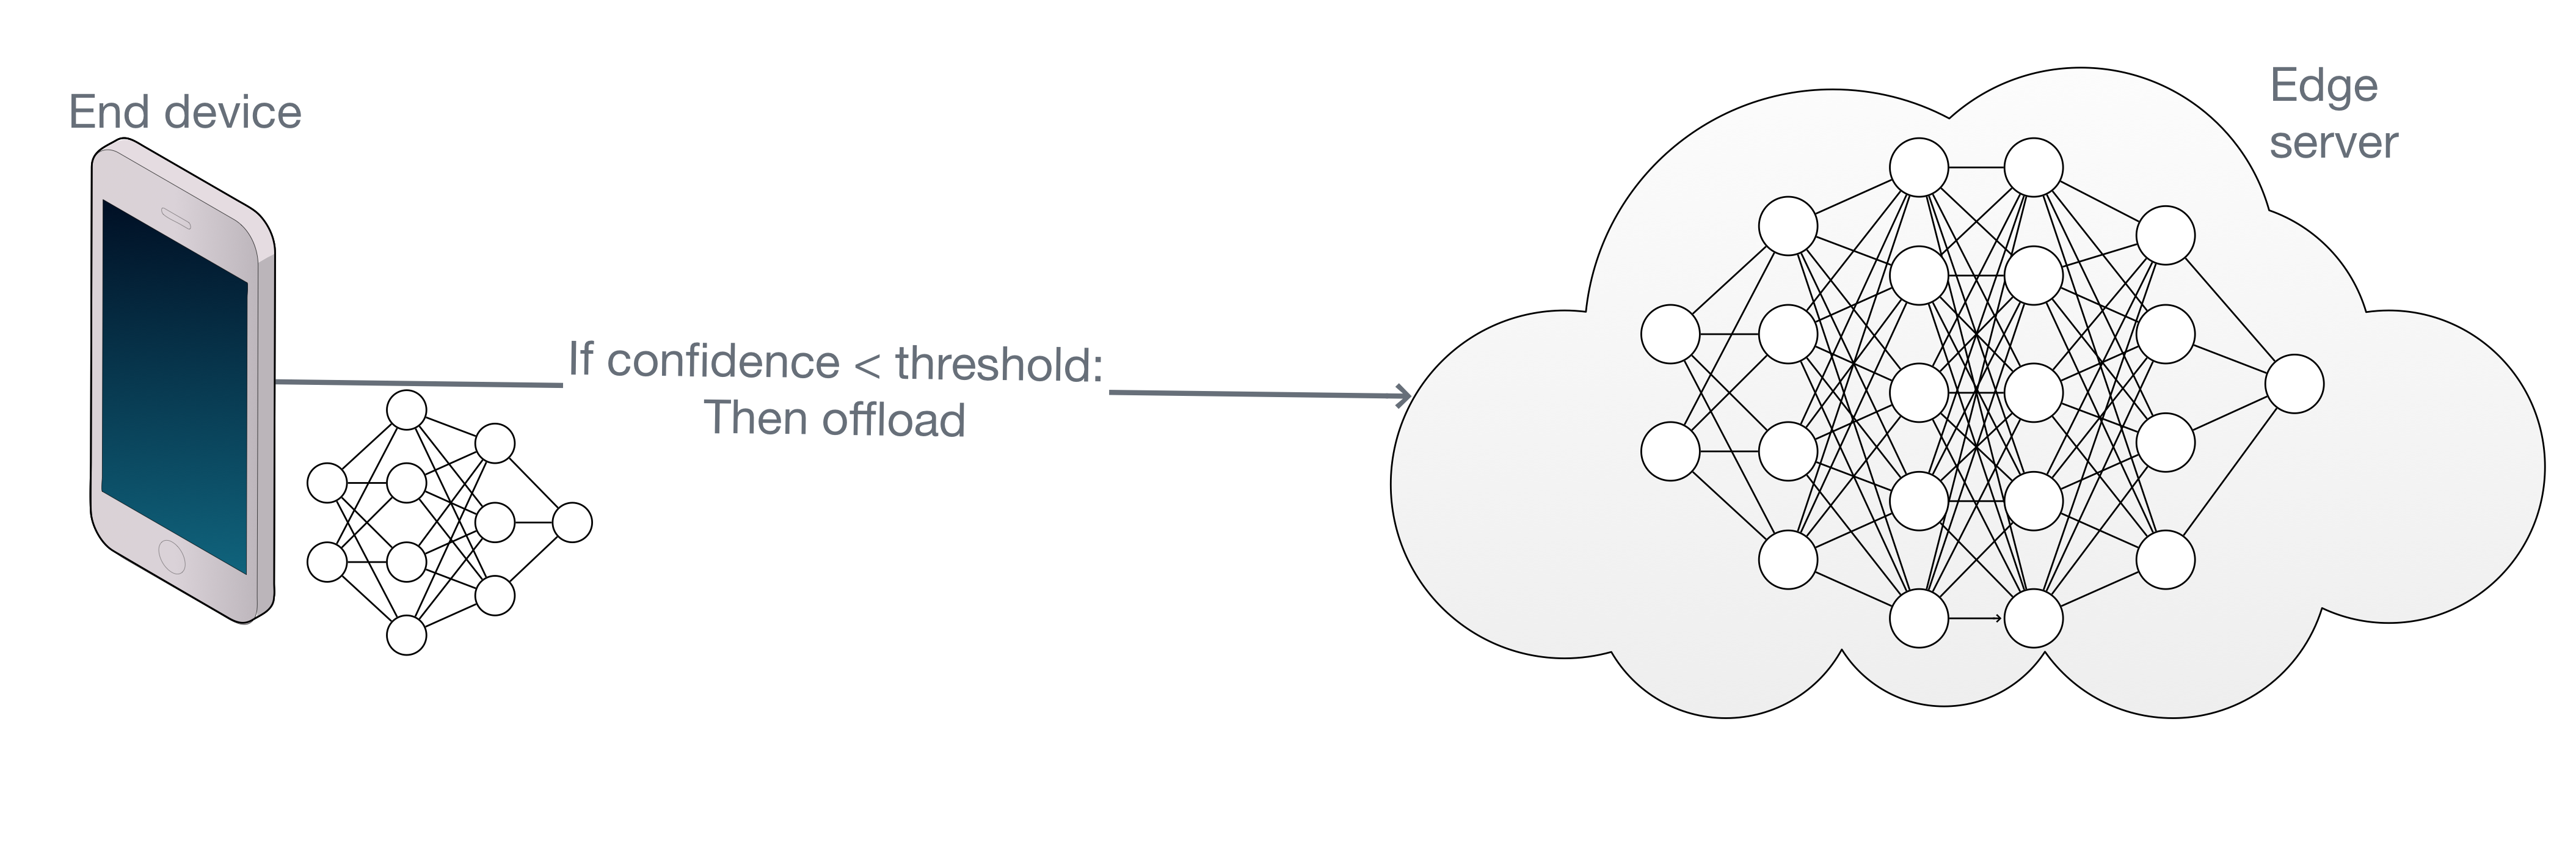
\includegraphics[width=.8\linewidth]{figures/models/big_little_dnn}
		\captionof{figure}[Big/Little \gls{dnn} architecture]{Big/Little \gls{dnn}, a hybrid edge architecture. An on-device model is used to selectively offload to a more complex model hosted on an edge server.}
		\label{fig:big/little-dnn}
	\end{minipage}
	
	A decision is made to offload for big model inference on the edge server if the confidence of the prediction of the little model is unsatisfactory. If a lot of samples can be correctly classified locally, a speed-up is gained by avoiding running an unnecessarily deep model, and costly unnecessary communication is spared. Still, the down-side of this approach is computation is wasted on the on-device inference of the little model if too many samples require the big model to satisfy the threshold. 
	
	\item[Model Early Exit] Cascading \gls{dnn} \cite{leroux_resource-constrained_2015} and \gls{branchynet} \cite{teerapittayanon_branchynet:_2016} are both early exiting frameworks for fast inference using \gls{dnn}s. Both studies show that only a few numbers of samples require extremely deep models to be correctly classified. The frameworks, illustrated in figure \ref{fig:branchynet}, adds intermediate classifiers, or branch exits to the \gls{dnn}. The intermediate classifiers allow samples that can achieve a score higher than a threshold to exit the inference process early. Other samples may require more layers or perhaps the entire depth of the model to get a high enough score. If a high threshold is selected, only a few samples might be able to exit the model. Thus no significant reduction in inference time is found. If a low threshold, a lot of samples will exit the model prematurely hence be incorrectly classified and degrade the accuracy. 
	
	\begin{minipage}[t]{\linewidth}    
		\centering                          
		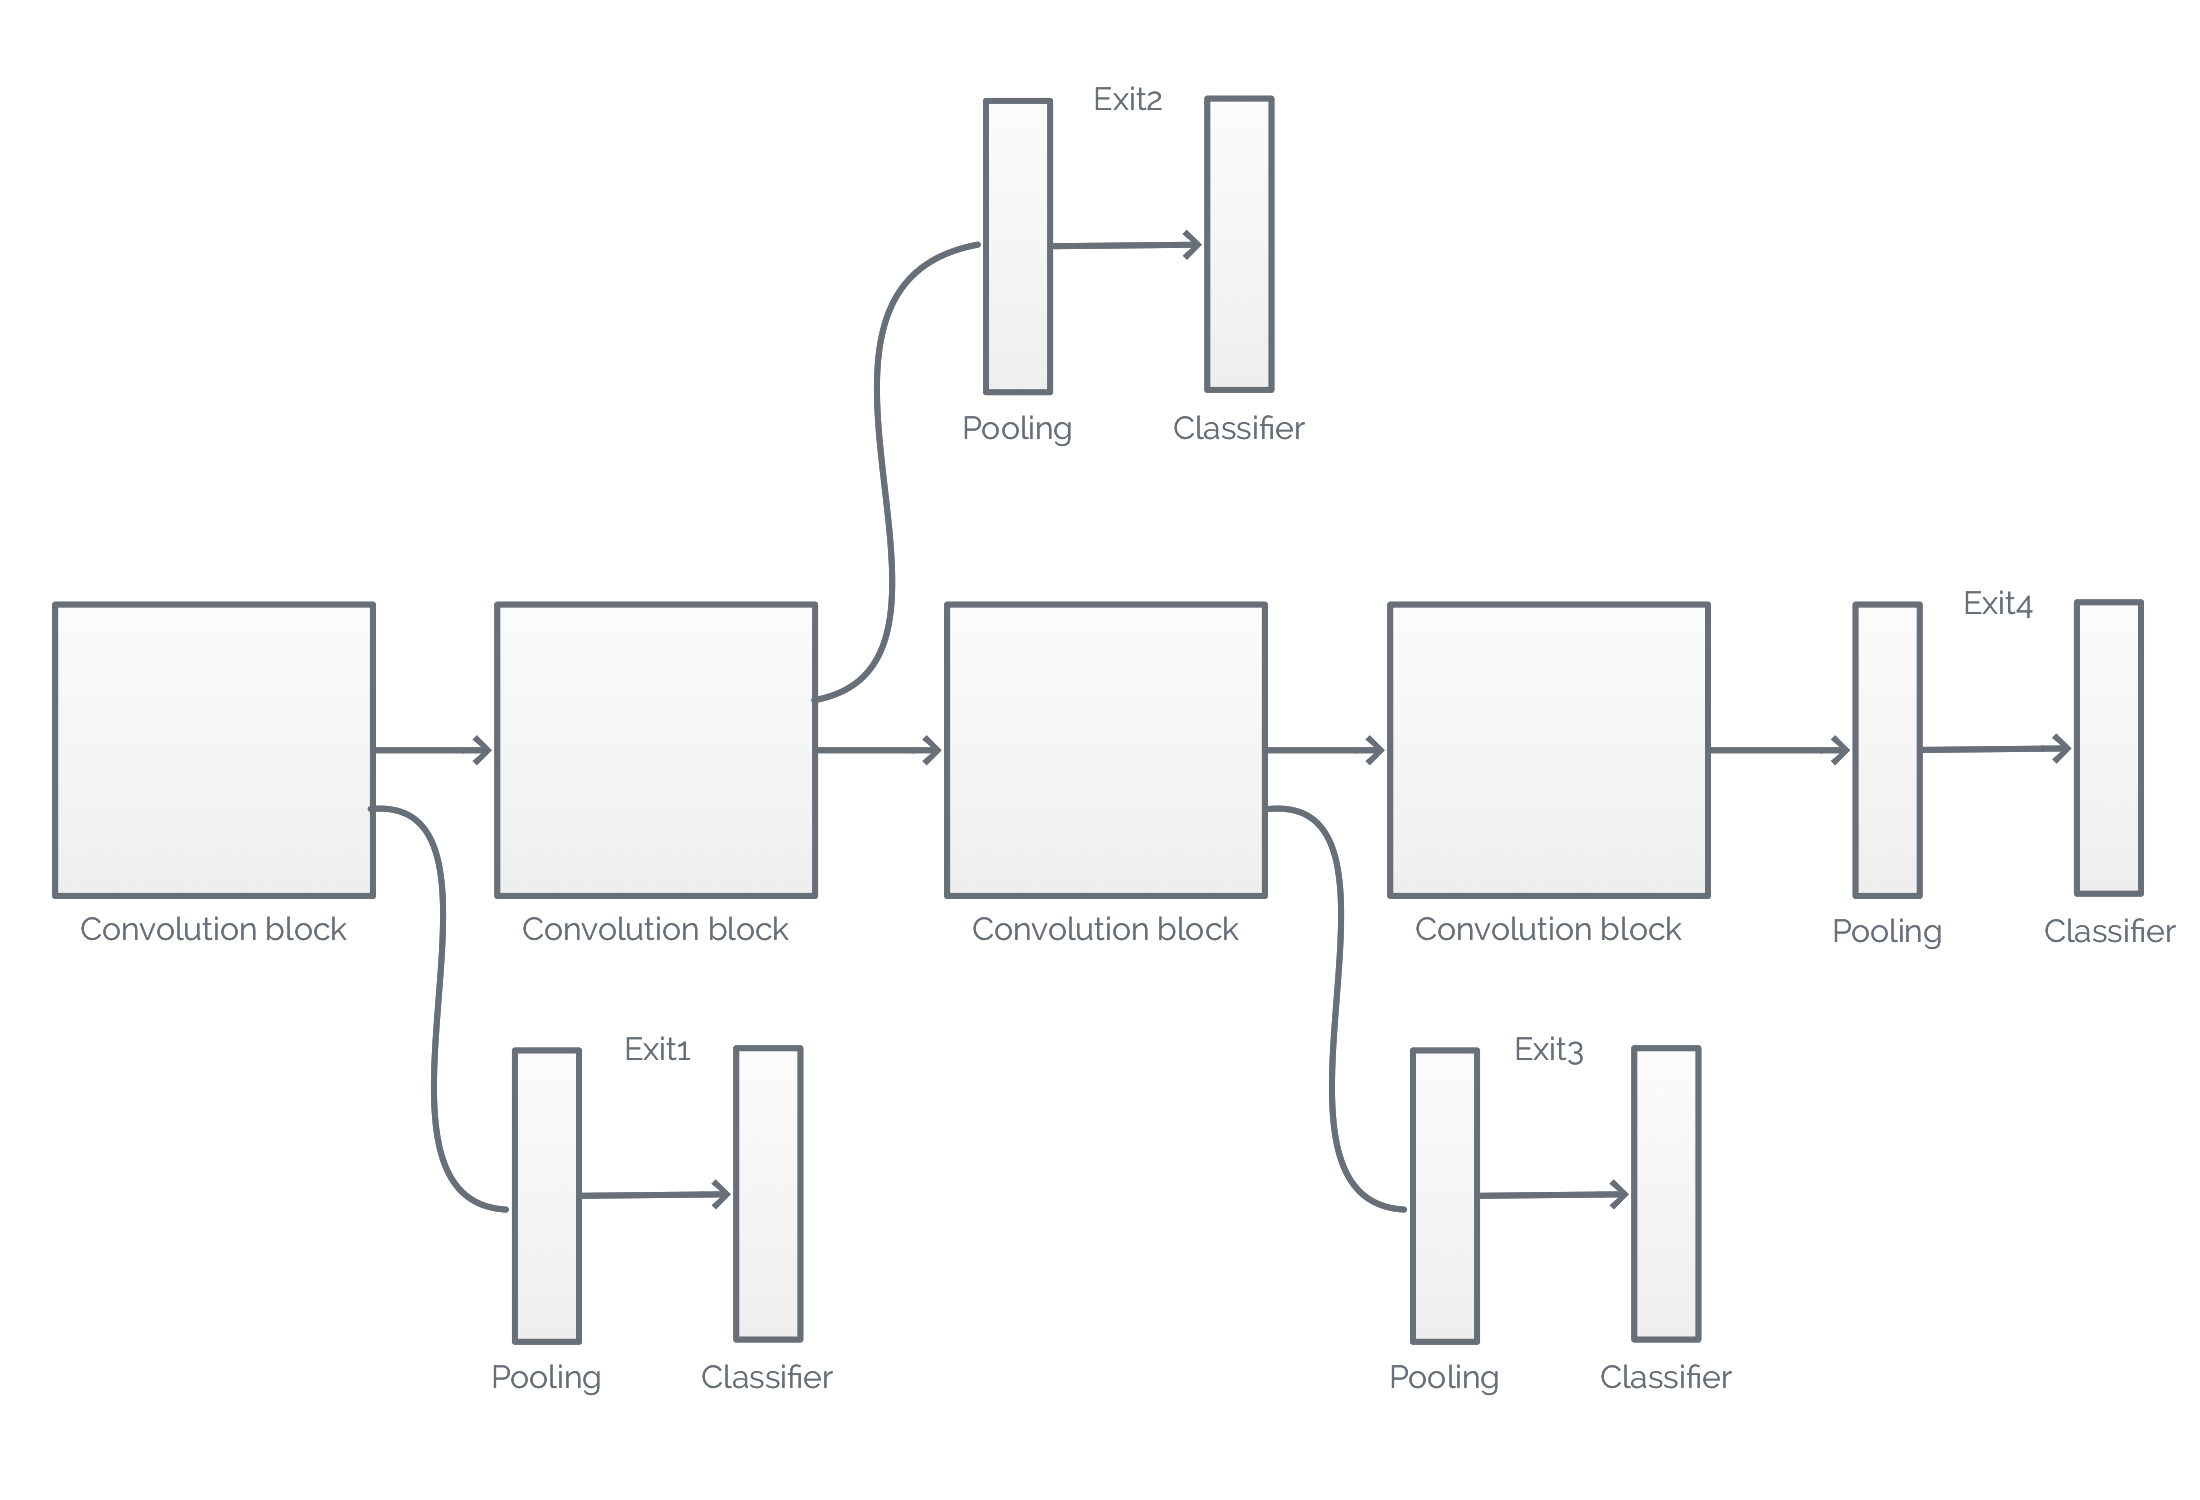
\includegraphics[width=.7\linewidth]{figures/models/branchy}
		\captionof{figure}[Early Exit Architecture]{Early Exit Architecture. Intermediate exits are added to the \acrfull{dag}.}
		\label{fig:branchynet}
	\end{minipage}
	
	\item[Model Layer Skipping] Research in \cite{wang_skipnet:_2017, wu_blockdrop:_2017}  have shown that layers of a \gls{dnn} can be skipped to reduce inference latency without sacrificing accuracy. SkipNet \cite{wang_skipnet:_2017} is a framework for adding dynamic decision for layer skipping. 
	
	\begin{minipage}[t]{\linewidth}    
		\centering                          
		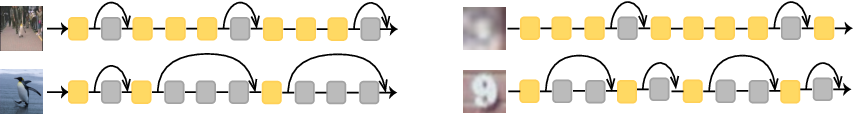
\includegraphics[width=.8\linewidth]{figures/models/skipnet}
		\captionof{figure}[SkipNet]{In SkipNet, layers are skipped depending on the complexity of the input. Source \citetitle{wang_skipnet:_2017} \cite{wang_skipnet:_2017}}
	\end{minipage}
	
	The framework adds complexity to the model by introducing skipping gates between intermediate layers of the network. The classifications are learned as a usual supervised learning problem using labeled data. Skipping-policies are learned using reinforcement learning by rewarding skipping decisions with a small impact on accuracy. The work shows that only a small fraction of inputs require these extremely deep models. Thus SkipNet can reduce the computational cost by 30\% of a\gls{resnet}101 on the ImageNet dataset. 
	
	BlockDrop \cite{wu_blockdrop:_2017} is another approach to learn skipping-policies. Instead of adding intermediate skipping gates for dynamic local decisions as in SkipNet. The training shows which classes are easy and which are hard. BlockDrop trains a global policy network and is similarly trained using reinforcement learning.  The policy network selectively chooses which model layers to use. BlockDrop can be regarded as a learned model selection framework, where the selection of models is learned by the policy network to estimate the complexity of an input sample. 
	
	
	\begin{minipage}[t]{\linewidth}    
		\centering
		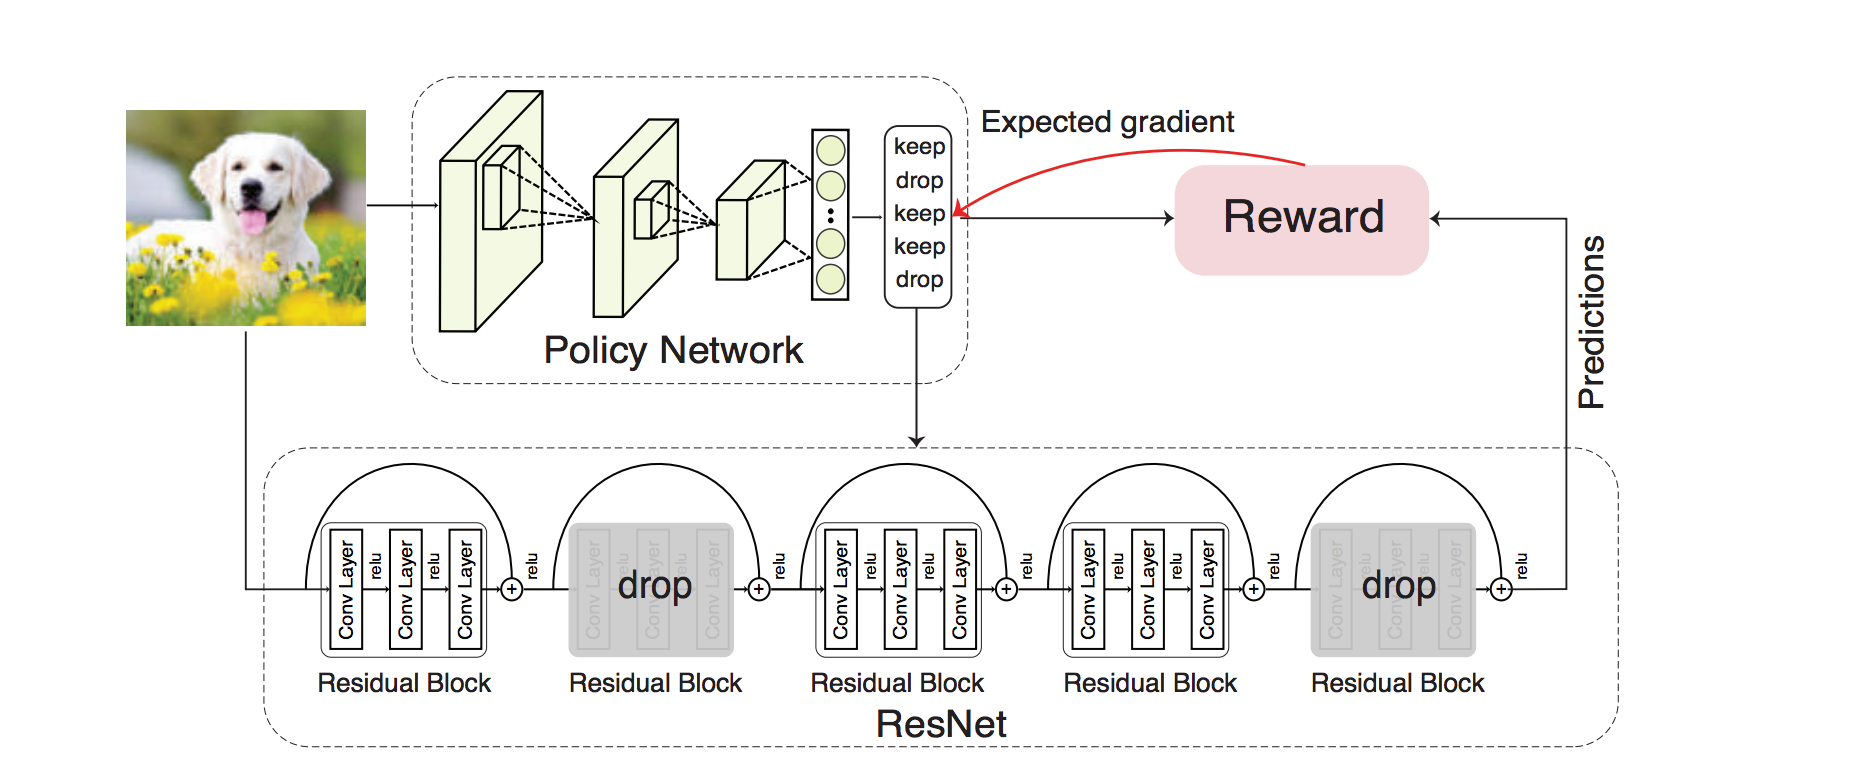
\includegraphics[width=\linewidth]{figures/models/blockdrop}
		\captionof{figure}[BlockDrop]{In BlockDrop, a policy network is trained to estimate the complexity of the input. Based on the complexity, a decision is made of which layer of a residual network to drop. Source \citetitle{wu_blockdrop:_2017} \cite{wu_blockdrop:_2017}}
	\end{minipage}	
	
	
\end{enumdescript}

\subsection{Collaborative Inference}

Collaborative inference of a \gls{dnn} is also known as model partitioning. Instead of solely executing a \gls{dnn} in the cloud, edge, or on-device, the computing resources collaborate to boost inference time. Splitting a model is an inherent nature of sequential \gls{dnn}s. The inference process can be stopped at any layer. The intermediate output after the last executed layer are transferred over the network, and the inference continues at the next layer on an edge server, as shown in figure \ref{fig:offlaoding}.

\begin{minipage}[t]{\linewidth}    
	\centering
	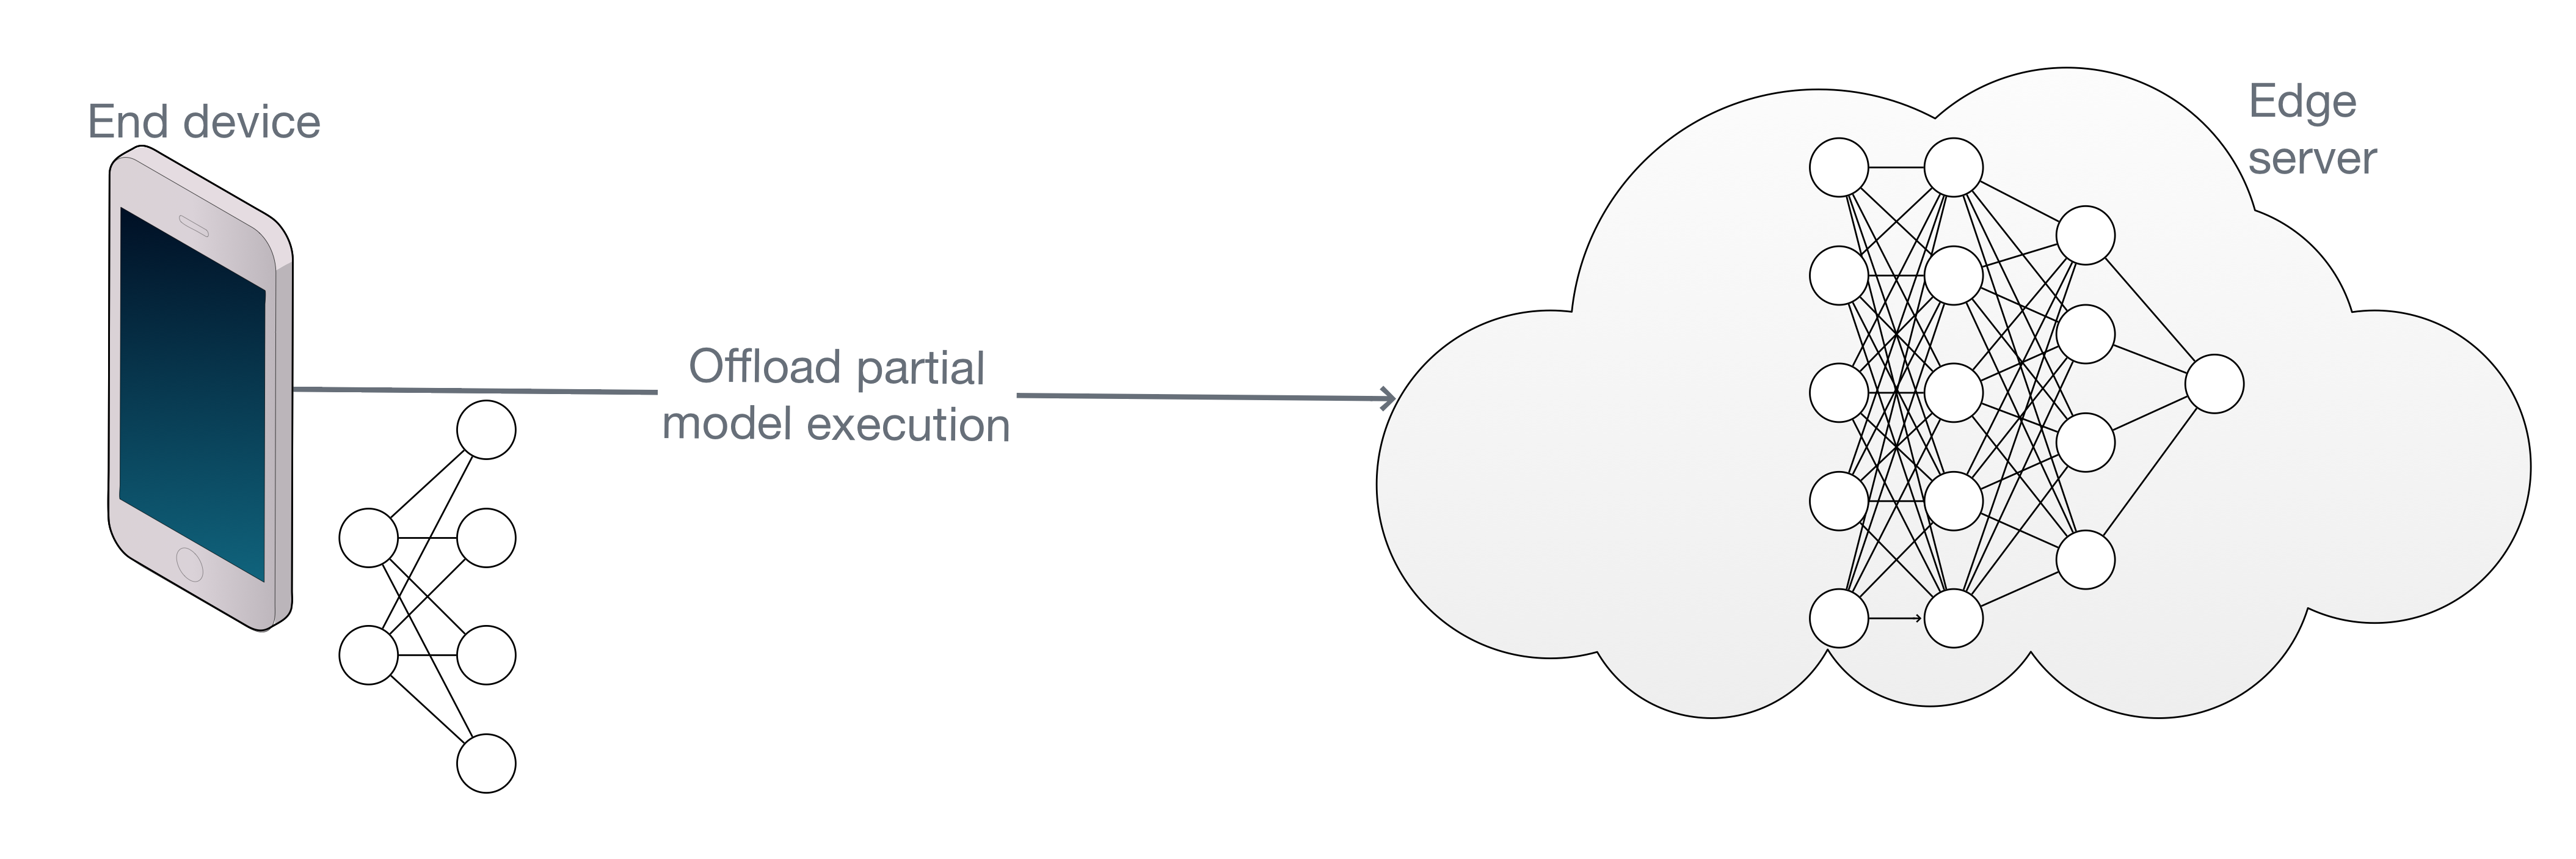
\includegraphics[width=\linewidth]{figures/models/partitioning}
	\captionof{figure}[Model partitioning]{For model partitioning, a part of the model is inferred on-device. The inference of the remaining layers is offloaded to the edge for processing.}
	\label{fig:offlaoding}
\end{minipage}

Neurosurgeon \cite{kang_neurosurgeon:_2017} is a lightweight partitioning scheduler. It constructs regression models for per layer execution time, and output data size of the \gls{dnn}. The regression models are used to decide the best partition of the \gls{dnn} based on the available communication data rate. The work is based on cloud-offloading and shows, that the conventional cloud-only approach is insufficient, due to low data rate connections with high variability to cloud data centers. Communication delay is the bottleneck in such an offloading application, hence a smaller representation of the input data is needed. However, the layers producing a smaller output than the original input typically lies deep within the network.
\begin{enumdescript}
	\item[Feature Compression] 
	
	Studies have been conducted to reduce the data volume to be transferred over the network when partitioning \gls{dnn}s to run in a collaborative scheme.  In \cite{choi_deep_2018}, they study the compression of intermediate features before transferring. They show that lossless compression has no impact on accuracy. However, the bit saving is also limited. Lossy compression, on the other hand, results in 70\% bit savings but also harm model accuracy. Compression aware training is proposed to compensate. In \cite{choi_near-lossless_2018}, they propose a novel compression technique, specially designed for deep features, i.e., the output of an intermediate \gls{dnn} layer. The compression of deep features shows significantly higher bit savings compared to conventional image compression algorithms such as JPEG. Alternatively, methods such as \gls{bottlenet} \cite{eshratifar_bottlenet:_2019}  proposes a novel \gls{dnn} module to limit the communication overhead.
	
	
	%	\begin{minipage}[t]{\linewidth}    
	%		\centering
	%		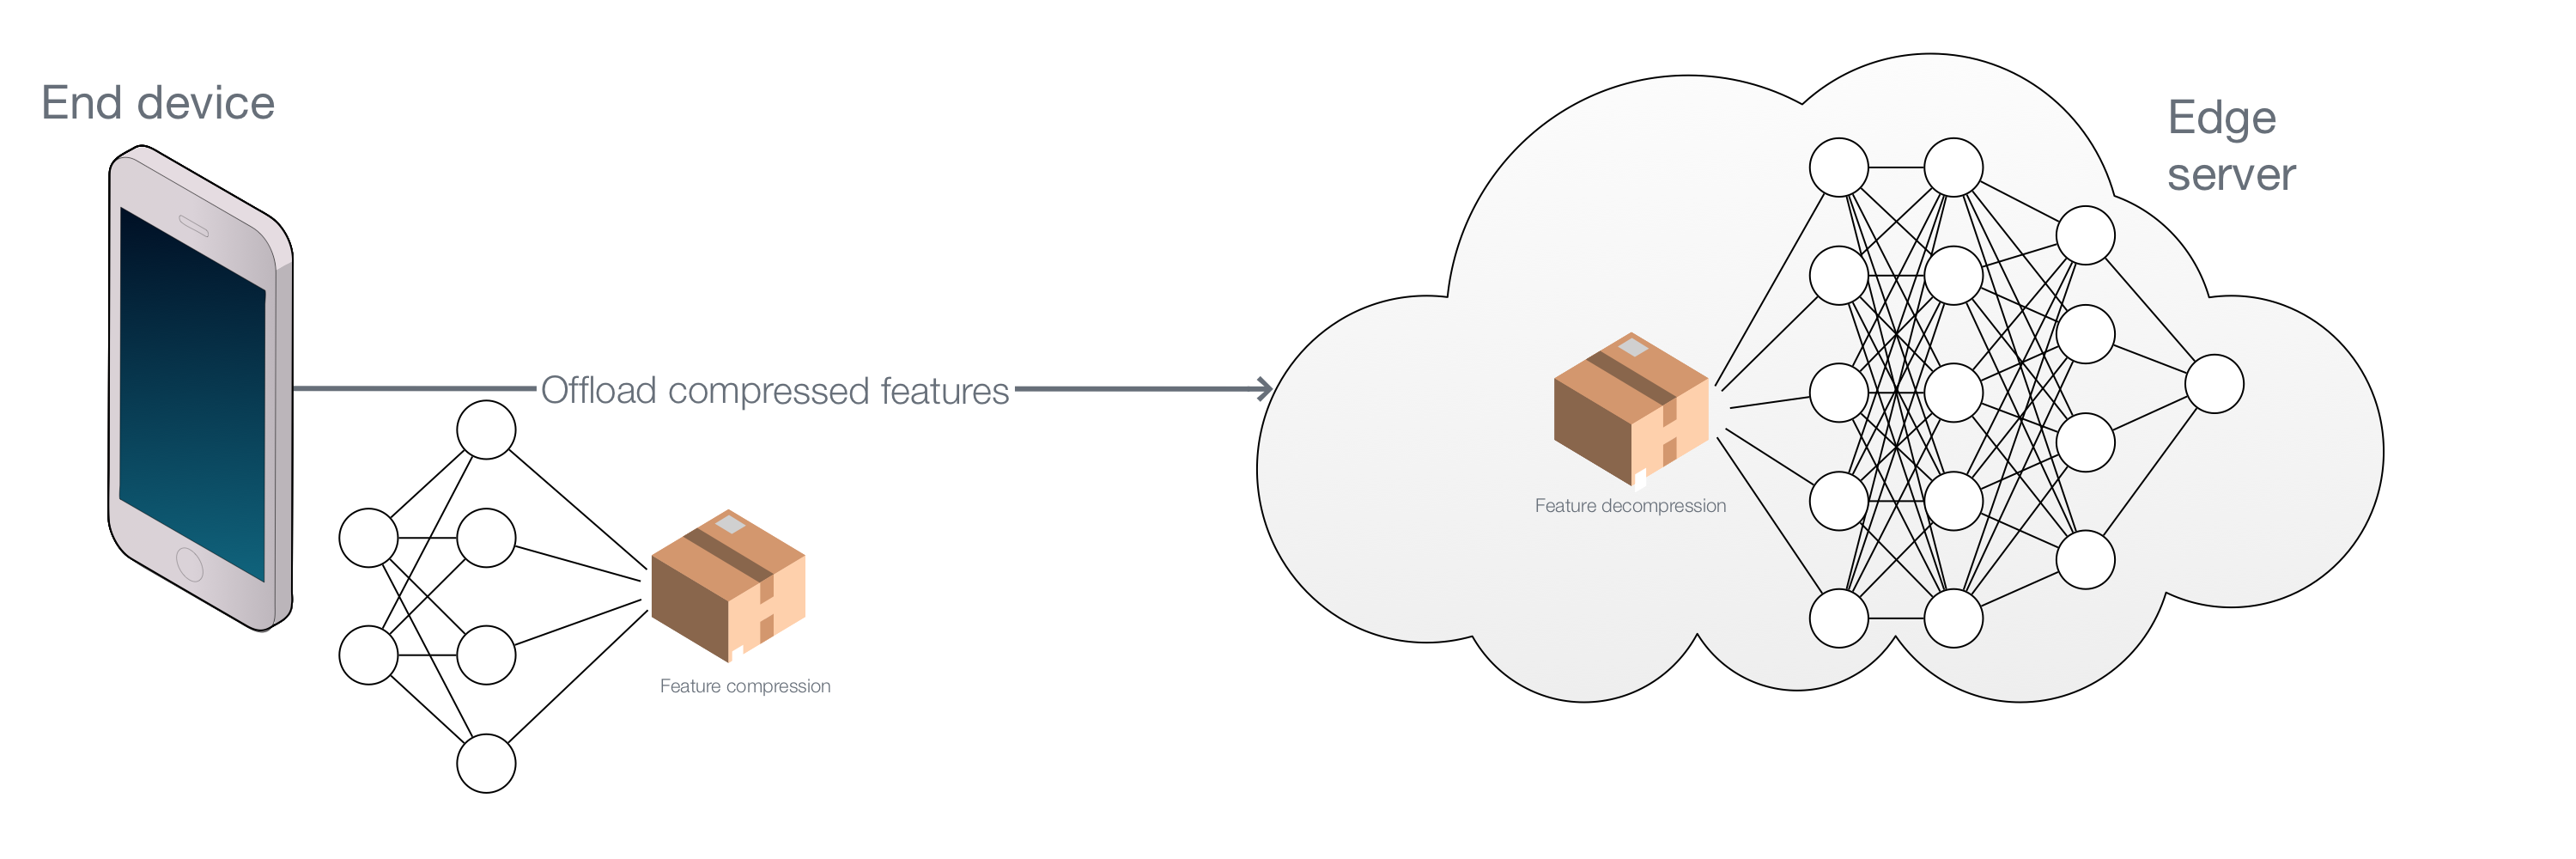
\includegraphics[width=\linewidth]{figures/models/compressed}
	%		\captionof{figure}[Feature compression]{Feature compression}
	%	\end{minipage}
	
	%	\gls{bottlenet} is a novel neural network module.
	Client-side \gls{bottlenet} implements a reduction unit and a compressor unit. The reduction unit creates a smaller representation of the intermediate features by applying spatial-wise and channel-wise convolutions. The compressor applies lossy JPEG compression to the features. The server decompresses the received data, and the restoration unit restores the intermediate feature using channel-wise and spatial-wise deconvolution.	
	
	\begin{minipage}[t]{\linewidth}
		\centering
		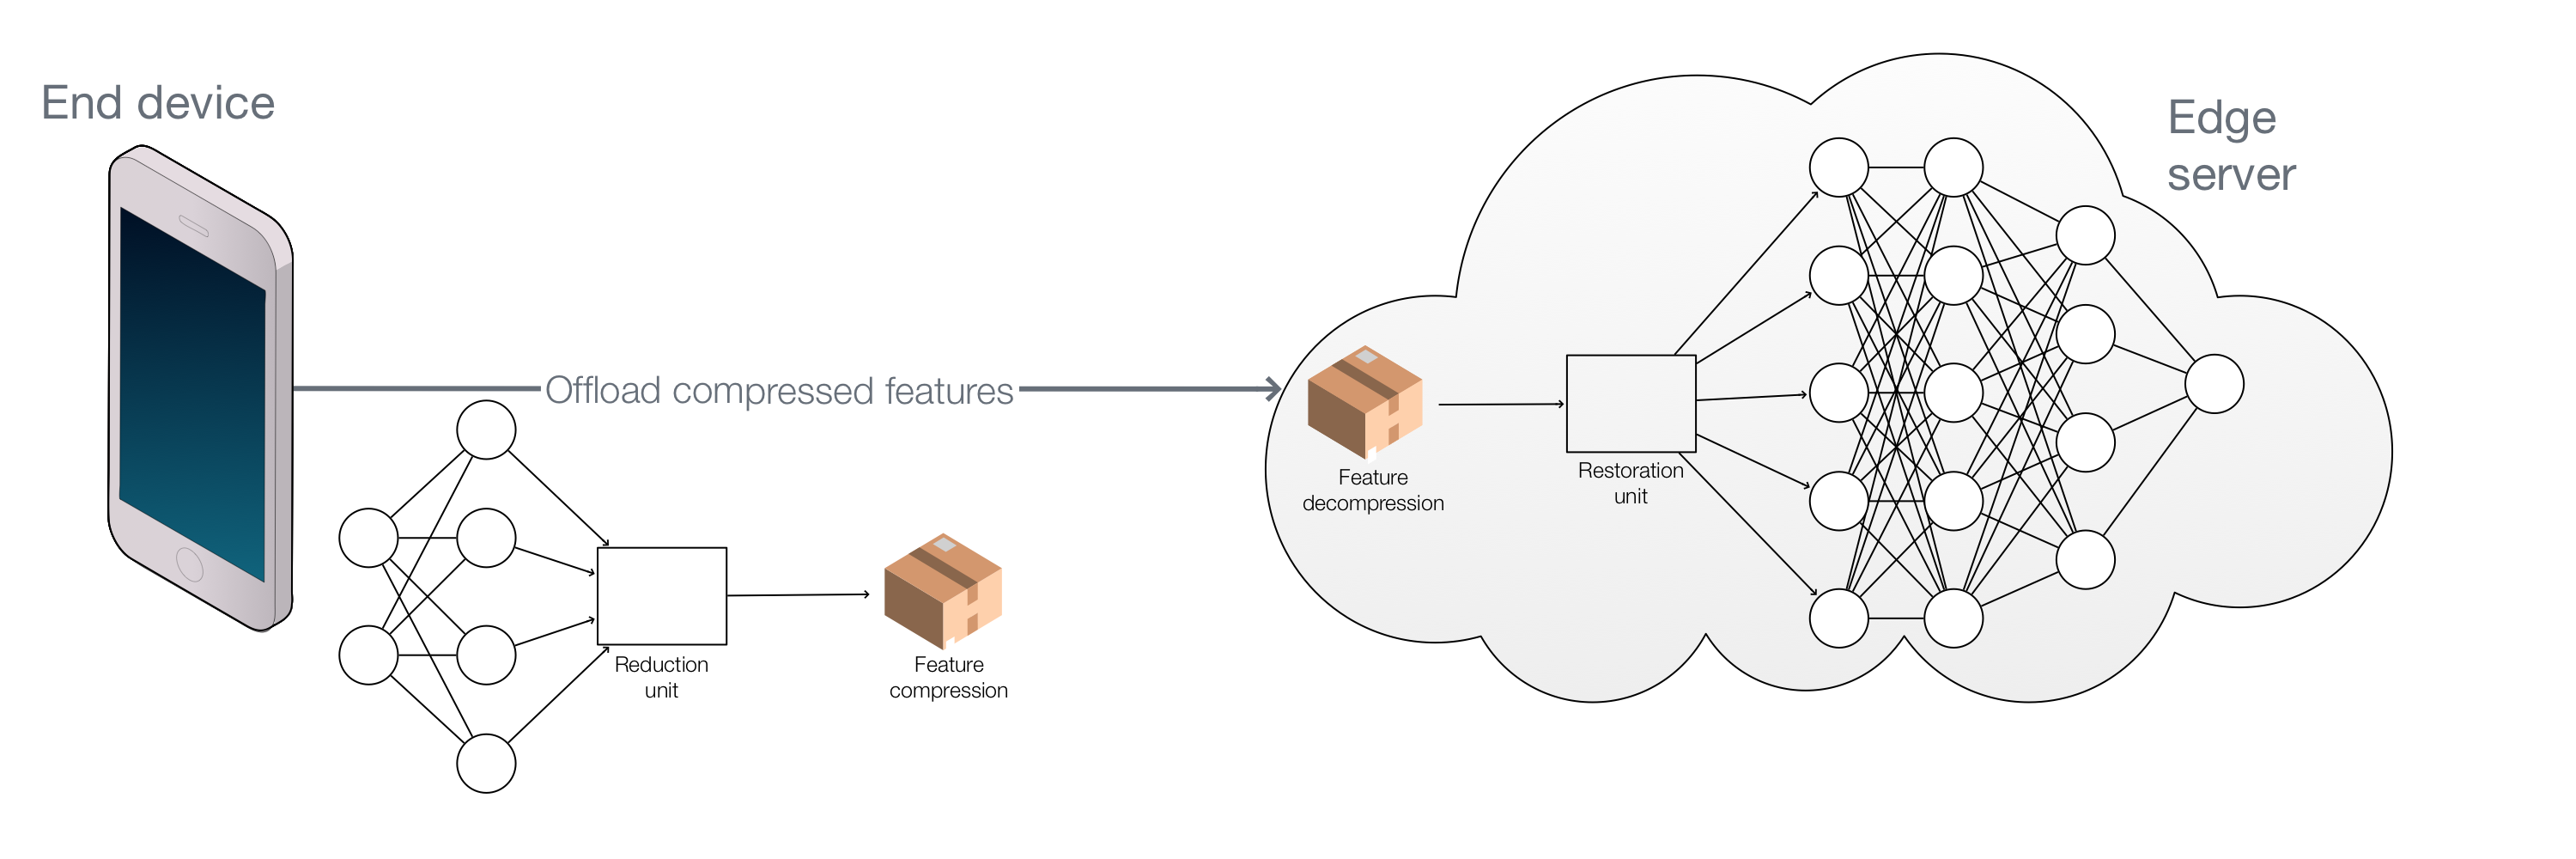
\includegraphics[width=.8\linewidth]{figures/models/bottlenet}
		\captionof{figure}[BottleNet Unit]{In BottleNet, the input size is reduced using spatial- and channel-wise convolutions and compressed using lossy compression. The input is restored server-side to continue the inference process.}
	\end{minipage}
	
	\gls{bottlenet} can achieve 84$\times$ bit savings compared offloading the entire image with less than 2\% degradation of accuracy. The deterioration is caused by lossy compression and compensated by compression-aware training. Under good networking conditions, the evaluation of \gls{bottlenet} shows that the best partition point is right after the first convolution, as a smaller representation of the input can already be found. 	
	\item[Distributed Exits] In \cite{leroux_cascading_2017,teerapittayanon_distributed_2017}, it is proposed to distribute early exit models over the network in a computing hierarchy on end-device, edge, and cloud. Figure \ref{fig:early-exit-colab} illustrates a partitioned early exit \gls{dnn} for the collaborative edge. 
	
	\begin{minipage}[t]{\linewidth}
		\centering
		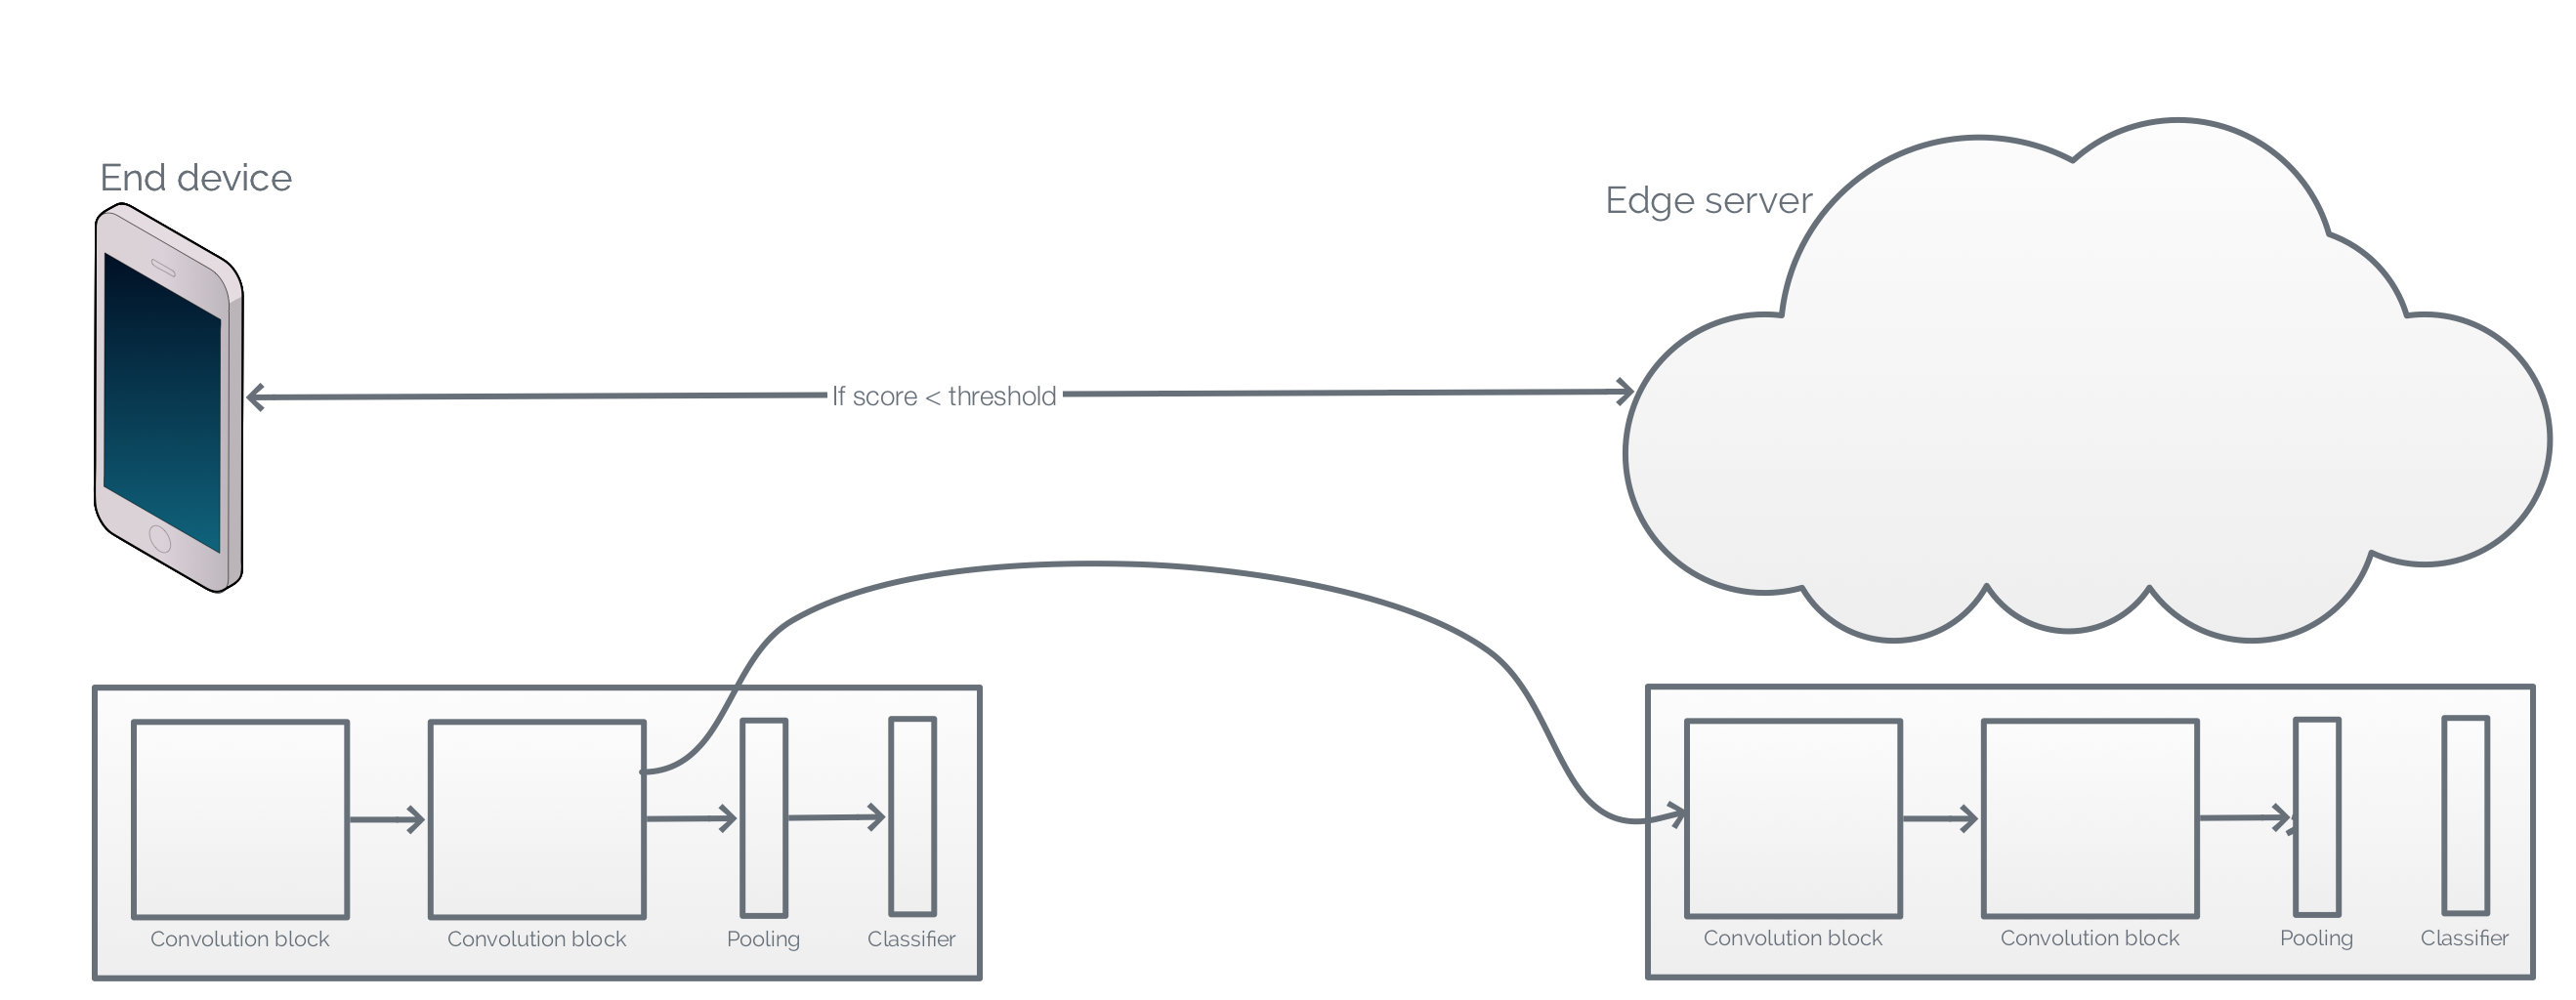
\includegraphics[width=\linewidth]{figures/models/cascaded}
		\captionof{figure}[Cascaded \gls{dnn} over a computing hierarchy]{A distributed exit model is partitioned to let a client handle the first or first couple of exit, and offload the remaining inference to one or more servers.}
		\label{fig:early-exit-colab}
	\end{minipage}

	The model is distributed in a manner, where one or more exits are processed by the end-device and one or more exits on the edge server. Communication efforts can be reduced by terminating the process locally if a satisfying prediction is obtained. Nonetheless, model partitioning introduces communication delay to the inference task that must be accounted for, e.g., using one of the methods for feature compression.
	
	\gls{ddnn} \cite{teerapittayanon_distributed_2017} extends the idea by proposing a framework for geographically distributed end-devices to solve an inference task collaboratively. It is decided to exit the inference locally if a satisfactory prediction score is obtained. If not, the intermediate outputs from the geographically distributed end-devices are aggregated for sensor fusion by a \gls{dnn} at a higher level in the hierarchy. The fusing \gls{dnn} produces a prediction using data from all upstream end-devices. Using the early exit model in this fashion does not only show improvement for early exits but also the final prediction. Additionally, \gls{ddnn}s offer benefits from distributed computing to provide fault tolerance, when some local \gls{dnn} comes with a poor or a missed prediction. \gls{ddnn} has been proposed for Industry 4.0 to solve autonomous defect detection in \cite{li_deep_2018}. 
	
	Distributed early exit models are used by Edgent \cite{li_edge_2018} to handle the latency-accuracy trade-off for time-critical application with a predefined deadline. Edgent is an optimization engine based on a deadline, a regression model of inference time of each layer, and the observed available bandwidth between end-device and edge server. Edgent makes a decision, to right-size the model by a selection of an optimal exit point, and to partition the model for collaboratively inference on end-device and edge by selecting a partitioning point. Edgent has shown to be able to meet more stringent deadlines, than running \gls{branchynet} solely on device or on edge.
\end{enumdescript}

\subsection{Distributed Inference}

The distributed inference is similar to collaborative inference. However, instead of partitioning the model in the depth-axis, i.e., between two layers, distributed inference partitions in the input-axis, i.e., have multiple peers collaborate to solve single layers. \gls{modnn} \cite{mao_modnn:_2017} is a framework to distribute the computing of the input to multiple worker nodes. Distributing computation input-wise can result in a higher degree of data dependence and lead to a higher degree of communication between workers. \gls{modnn} shows improvements in computing a \gls{dnn} inference on multiple mobile devices connected on a WLAN, compared to standalone inference on a single mobile device. DeepThings \cite{zhao_deepthings:_2018} is a framework intended for constraint \gls{iot} devices to distribute computation. In DeepThings, they take advantage of local region dependency in layers to split into multiple tasks. Due to dependency across layers, the task of the local region can be continued for the next layer. In this manner, they split the network layers horizontally but stack the work vertically, i.e., creating multiple thinner \gls{dnn}s working on local regions.
